%!TEX root = IAL.tex

\chapter{Sistemas Lineares}

Ao longo de todo esse capítulo o conjunto $\cp{K}$ será considerado como sendo um dos conjuntos: $\rac$, $\real$ ou $\complex$.

\section{Sistemas Lineares}\label{ssub:sistemas_lineares}
Vamos trabalhar com \textbf{equações lineares}\index{Sistema linear!equação linear} em $n$ variáveis $x_1$, $x_2$, \dots, $x_n$ que são equações que podem ser escritas na forma
\begin{equation}\label{equacao_linear}
    a_1x_1  + a_2x_2 +  \cdots + a_qx_q  = b,
\end{equation}
onde $a_1$, $a_2$, \dots, $a_q$, $b$ são escalares no corpo $\cp{K}$, sendo que nem todos os coeficientes $a_i$ são nulos.

No caso em que $b = 0$,  a equação \eqref{equacao_linear} tem a forma
\begin{equation}
    a_1x_1 + a_2x_2 + \cdots + a_qx_q = 0
\end{equation}
e é chamada de uma \textbf{equação linear homogênea}\index{Sistema linear!equação linear homogênea}.

\begin{exemplos}
    \begin{enumerate}[label={\arabic*})]
        \item Equações da forma
            \begin{enumerate}
                \item $x_1 + 2x_2 - 3x_3 = 10$, em $\cp{K} = \rac$
                \item $2x_1 + 0x_2 + \sqrt{2}x_3 - 4x_4 = 0$, em $\cp{K} = \real$, que será escrita como $2x_1 + 0x_2 + \sqrt{2}x_3 - 4x_4 = 0$
                \item $ix_1 + (2 +i)x_2 = 3 + 2i$, em $\cp{K} = \complex$
            \end{enumerate}
        são exemplos de \textbf{equações lineares}.

        \item Já equações na forma
            \begin{enumerate}
                \item $x_1^2 + 2x_2 - 3x_3 = 0$ em $\cp{K} = \real$
                \item $x_1 + 2\sin(x_2) + 3x_3 + x_ 4 = 1$ em $\cp{K} = \real$
                \item $2x_1 + 3x_2 - 4x_3^{-1} = 2$ em $\cp{K} = \rac$
            \end{enumerate}
        não são equações lineares e portanto não serão abordadas nesse curso.
    \end{enumerate}
\end{exemplos}

Considerando $\cp{K} = \real$, queremos analisar um conjunto de equações lineares do tipo:

\begin{align}
    \begin{cases}\label{sistema_linear_2x2}
        ax + by = b_1\\
        cx + dy = b_2
    \end{cases}
\end{align}
onde $a$, $b$, $c$, $d$, $b_1$, $b_2 \in \cp{K}$.

Queremos saber se é possível encontrar valores para $x$, $y$ no conjunto $\real$ de modo que essas duas equações sejam simultaneamente verdadeiras? Caso existam, gostaríamos de determinar todos os possíveis valores que $x$ e $y$ podem assumir.

Observe que cada equação linear em \eqref{sistema_linear_2x2} representa uma reta no plano cartesiano. Assim queremos determinar se essas restas possuem alguma interseção.

Mas sabemos que duas retas no plano podem ser coincidentes, paralelas ou se interceptam em um único ponto.

Assim se as retas do sistema \eqref{sistema_linear_2x2} são \textbf{coincidentes}, existem infinitos valores de $x$, $y \in \cp{K}$ que satisfazem as duas equações simultaneamente. Neste caso dizemos que o sistema \eqref{sistema_linear_2x2} é \textbf{possível e indeterminado}.

\definecolor{qqqqff}{rgb}{0,0,1}
\definecolor{ffqqqq}{rgb}{1,0,0}
\begin{center}
    \begin{tikzpicture}[line cap=round,line join=round,>=triangle 45,x=1cm,y=1cm]
        \begin{axis}[
            x=1cm,y=1cm,
            axis lines=middle,
            xticklabels={,,},
            yticklabels={,,},
            xlabel=$x$,
            ylabel=$y$,
            xmin=-2,
            xmax=5,
            ymin=-1.3,
            ymax=3,]
            \draw [line width=5.2pt,dash pattern=on 1pt off 1pt,color=ffqqqq,domain=-1.348257839721257:5.807994044102577] plot(\x,{(--4-1*\x)/2});
            \draw [line width=2pt,color=qqqqff,domain=-1.348257839721257:5.807994044102577] plot(\x,{(--8-2*\x)/4});
            \begin{scriptsize}
                \draw[color=ffqqqq] (1.8,2) node {$a_{11}x + a_{12}y = b_1$};
                \draw[color=qqqqff] (3,1.5) node {$a_{21}x + a_{22}y = b_2$};
            \end{scriptsize}
        \end{axis}
    \end{tikzpicture}
\end{center}

Agora se as retas em \eqref{sistema_linear_2x2} são \textbf{paralelas}, não existem valores de $x$, $y \in \cp{K}$ satisfazendo as duas equações simultaneamente. Nesse caso dizemos que o sistema \eqref{sistema_linear_2x2} é \textbf{impossível}.

\definecolor{ffqqqq}{rgb}{1,0,0}
\definecolor{qqqqff}{rgb}{0,0,1}
\begin{center}
    \begin{tikzpicture}[line cap=round,line join=round,>=triangle 45,x=1cm,y=1cm]
        \begin{axis}[
            x=1cm,y=1cm,
            axis lines=middle,
            xticklabels={,,},
            yticklabels={,,},
            xlabel=$x$,
            ylabel=$y$,
            xmin=-5.3,
            xmax=6.3,
            ymin=-1,
            ymax=4.3,]
            \draw [line width=2pt,color=qqqqff,domain=-5:6] plot(\x,{(--4-1*\x)/5});
            \draw [line width=2pt,color=ffqqqq,domain=-5:6] plot(\x,{(--16-1*\x)/5});
            \begin{scriptsize}
                \draw[color=qqqqff] (-3.8,2.2) node {$a_{21}x + a_{22}y = b_2$};
                \draw[color=ffqqqq] (-3.8,3.4) node {$a_{11}x + a_{12}y = b_1$};
            \end{scriptsize}
        \end{axis}
    \end{tikzpicture}
\end{center}

Por fim, as retas em \eqref{sistema_linear_2x2} podem se \textbf{interceptar}. Nesse caso existe um único conjunto de valores $x = \alpha \in \cp{K}$ e $y = \lambda \in \cp{K}$ que satisfaz as duas equações simultaneamente. Neste caso dizemos que o sistema \eqref{sistema_linear_2x2} é \textbf{possível e determinado}.

\definecolor{qqqqff}{rgb}{0,0,1}
\definecolor{ffqqqq}{rgb}{1,0,0}
\begin{center}
    \begin{tikzpicture}[line cap=round,line join=round,>=triangle 45,x=1cm,y=1cm]
        \begin{axis}[
            x=1cm,y=1cm,
            axis lines=middle,
            xticklabels={,,},
            yticklabels={,,},
            xlabel=$x$,
            ylabel=$y$,
            xmin=-2,
            xmax=4.3,
            ymin=-2,
            ymax=3.5,]
            \draw [line width=2pt,color=ffqqqq,domain=-4:5] plot(\x,{(--4.94--7.92*\x)/7.58});
            \draw [line width=2pt,color=qqqqff,domain=-4:5] plot(\x,{(--4.824-8.66*\x)/8.24});
            \begin{scriptsize}
                \draw[color=ffqqqq] (2.9,2) node {$a_{11}x + a_{12}y = b_1$};
                \draw[color=qqqqff] (2.7,-0.5) node {$a_{21}x + a_{22}y = b_2$};
            \end{scriptsize}
        \end{axis}
    \end{tikzpicture}
\end{center}

Esse mesmo tipo de análise pode ser aplicada num sistema da forma
\begin{align}
    \begin{cases}\label{sistema_linear_3x3}
        a_1x + a_2y + a_3z = b_1\\
        a_4x + a_5y + a_6z = b_2\\
        a_7x + a_8y + a_9z = b_3
    \end{cases}
\end{align}
onde $a_i \in \cp{K}$ para $1 \le i \le 9$ e $b_j \in \cp{K}$ para $1 \le j \le 3$.

Neste caso as equações desse sistema representam planos no espaço tridimensional. Nesse sistema então queremos saber quais são as possíveis interseções entre estes três planos.

Temos então as seguintes possibilidades:

\begin{enumerate}
    \item Os três planos se interceptam em um único ponto. Assim existe um único conjunto de valores $x = \alpha \in \cp{K}$, $y = \lambda \in \cp{K}$ e $z = \gamma \in \cp{K}$  que satisfaz as três equações simultaneamente.  Neste caso dizemos que o sistema \eqref{sistema_linear_3x3}  é \textbf{possível e determinado}.
        \begin{figure}[h]
            \centering
            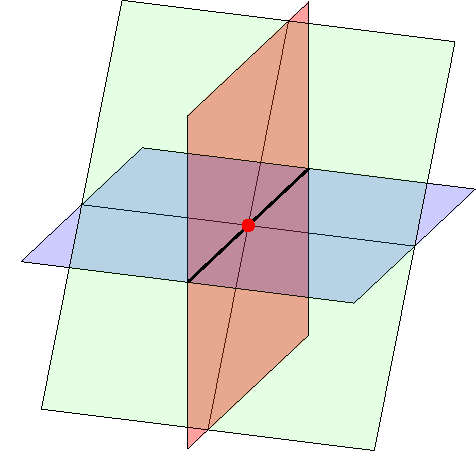
\includegraphics[scale=0.6]{3-planos-solucao-unica.pdf}
                \caption{Solução única}
        \end{figure}
    \item Os três planos se interceptam em infinitos pontos. Existem infinitos valores de $x$, $y$, $z \in \cp{K}$ que satisfazem as três equações simultaneamente. Neste caso dizemos que o sistema \eqref{sistema_linear_3x3} é \textbf{possível e indeterminado}.
        \begin{figure}[h]
            \centering
            \begin{subfigure}{.32\textwidth}
                \centering
                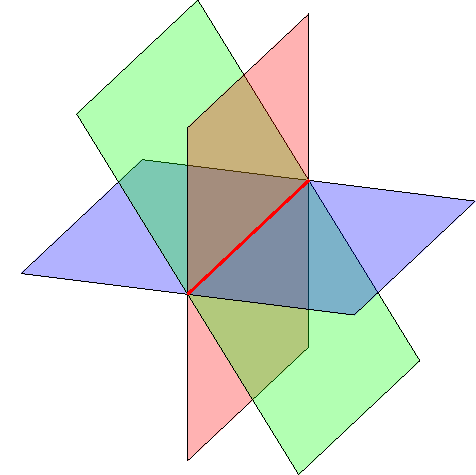
\includegraphics[width=\linewidth]{2-planos-coincidentes-infinitas-solucoes-intersecao-reta.pdf}
                \caption{Infinitas soluções}
            \end{subfigure}
            \begin{subfigure}{.32\textwidth}
                \centering
                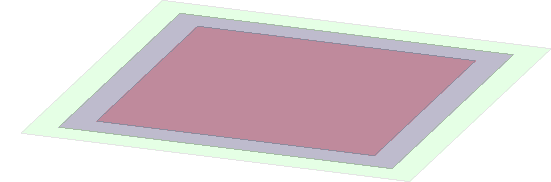
\includegraphics[width=\linewidth]{3-planos-coincidentes-infinitas-solucoes.pdf}
                \caption{Infinitas soluções}
            \end{subfigure}
            \begin{subfigure}{.32\textwidth}
                \centering
                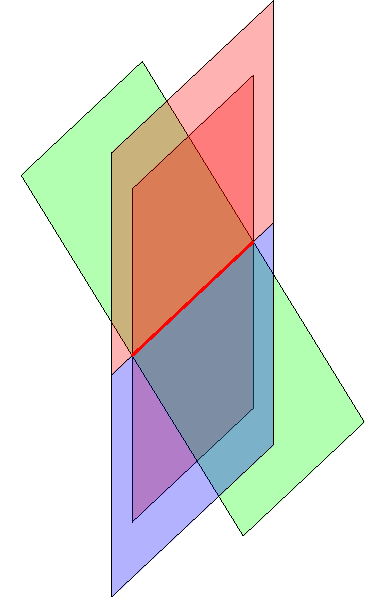
\includegraphics[width=\linewidth]{2-planos-coincidentes-terceiro-fora-infinitas-solucoes-intersecao-reta.pdf}
                \caption{Infinitas soluções}
            \end{subfigure}
        \end{figure}
    \item Os três planos não possuem uma interseção em comum. Neste caso não existem valores de $x$, $y$, $z \in \cp{K}$  satisfazendo as três equações simultaneamente. Assim dizemos que o sistema \eqref{sistema_linear_3x3}  é \textbf{impossível}.
        \begin{figure}[h]
            \centering
            \begin{subfigure}{.32\textwidth}
                \centering
                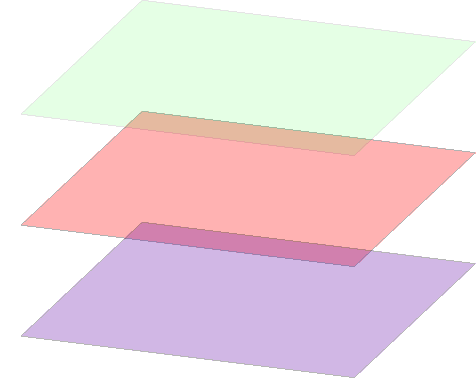
\includegraphics[width=\linewidth]{3-planos-paralelos-nenhuma-solucao.pdf}
                \caption{Nenhuma solução}
            \end{subfigure}
            \begin{subfigure}{.32\textwidth}
                \centering
                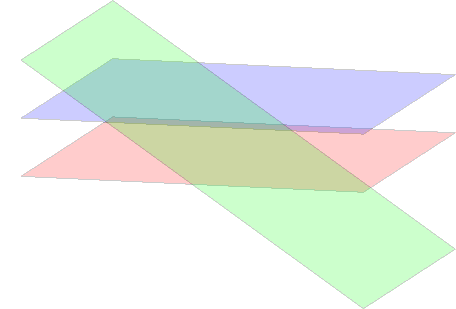
\includegraphics[width=\linewidth]{2-planos-paralelos-nenhuma-solucao.pdf}
                 \caption{Nenhuma solução}
              \end{subfigure}
            \begin{subfigure}{.32\textwidth}
                \centering
           
\includegraphics[width=\linewidth]{3-planos-sem-nenhuma-intersecao-dois-a-dois-retas-nenhuma-solucao.pdf}
            \caption{Nenhuma solução}
           \end{subfigure}
        \end{figure}
\end{enumerate}

Agora, de modo geral queremos trabalhar com uma quantidade qualquer de equações. Para isso começamos escolhendo escalares $b_1$, \dots, $b_m$  e $a_{ij}$,  $1 \le i \le m$, $1 \le j \le n$ todos em $\cp{K}$.

Queremos saber se é possível encontrar valores para  $x_1$, $x_2$, \dots, $x_n$  de modo que o seguinte conjunto de equações sejam válidas:
\begin{equation}\label{sistema_linear_geral}
\begin{cases}
        a_{11}x_1 + a_{12}x_2 + \cdots + a_{1n}x_n = b_1\\
        a_{21}x_1 + a_{22}x_2 + \cdots + a_{2n}x_n = b_2\\
        \qquad \vdots\\
        a_{m1}x_1 + a_{m2}x_2 + \cdots + a_{mn}x_n = b_m
    \end{cases}
\end{equation}

O conjunto de equações em \eqref{sistema_linear_geral} é chamado de um  \textbf{sistema de $m$ equações lineares  a $n$ incógnitas}\index{Sistema linear} $x_1$, $x_2$, \dots, $x_n$ , ou simplesmente de um \textbf{sistema linear}, nas incógnitas  $x_1$, $x_2$, \dots, $x_n$.

Uma solução de um sistema linear do tipo \eqref{sistema_linear_geral}
\[
    x_1 = \alpha_1,  x_2 = \alpha_2,  \dots, x_n = \alpha_n
\]
onde $\alpha_1$, $\alpha_2$, \dots, $\alpha_n \in \cp{K}$,  pode ser escrita como
\[
    (\alpha_1, \alpha_2, \dots, \alpha_n)
\]
e é chamada de uma \textbf{ênupla ordenada}\index{Sistema linear!ênupla ordenada} ou uma \textbf{n-upla ordenada}.


Se $b_1 = b_2 = \cdots = b_m = 0_\cp{K} \in K$,  dizemos que o sistema
\begin{equation}\label{sistemalinearhomogeneo}
    \begin{cases}
        a_{11}x_1 + a_{12}x_2 + \cdots + a_{1n}x_n = 0_\cp{K}\\
        a_{21}x_1 + a_{22}x_2 + \cdots + a_{2n}x_n = 0_\cp{K}\\
        \qquad \vdots\\
        a_{m1}x_1 + a_{m2}x_2 + \cdots + a_{mn}x_n = 0_\cp{K}
    \end{cases}
\end{equation}
é um \textbf{sistema linear homogêneo}.\index{Sistema linear!homogêneo}

Observe que tal sistema sempre possui solução,  a saber, $x_1 = x_2 = \cdots = x_n = 0_\cp{K}$.

Para o caso de sistemas lineares temos o seguinte resultado:

\begin{teorema}
    Todo sistema linear do tipo \eqref{sistema_linear_geral} tem zero, uma ou uma infinidade de soluções. Não existem outras possibilidades.
\end{teorema}

No caso de um sistema linear da forma \eqref{sistema_linear_geral}, o processo para encontrar suas soluções será feito mediante o uso de 3 tipos de operações. São elas:
\begin{itemize}
\item[$e_1$)] Troca da posição de duas equações.
\item[$e_2$)] Multiplicação de uma equação por um escalar não nulo.
\item[$e_3$)] Substituição de uma equação pela soma desta equação com alguma outra.
\end{itemize}

Estas três operações são chamadas de  \textbf{operações elementares}.

\begin{exemplos}
    Utilizando somente operações elementares encontre as soluções dos seguintes sistemas lineares:
    \begin{enumerate}[label={\arabic*})]
        \item $\begin{cases}x + y = 4\\3x + 3y = 6\end{cases}$

        \item $\begin{cases}x + y + 2z = 9\\ 2x + 4y - 3z = 1\\ 3x + 6y - 3z = 0\end{cases}$
    \end{enumerate}

    \begin{solucao}
        \begin{enumerate}[label={\arabic*})]
            \item Neste caso podemos somar a segunda equação do sistema com ela mesma mais -3 vezes a primeira equação:
                \[
                    \begin{cases}
                        x + y = 4\\
                        3x + 3y + (-3x) + (-3y) = 4 + (-3)\cdot 4
                    \end{cases}
                \]
            que resulta em
            \[
                \begin{cases}
                    x + y = 4\\
                    0 = -6
                \end{cases}
            \]
            e a segunda equação desse sistema é uma contradição. Logo não existem valores para $x$ e $y$ em $\real$ que satisfazem as duas equações desse sistema simultaneamente. Portanto tal sistema é um \textbf{sistema impossível}.
                    \item Denote as linhas desse sistema por $L_1$, $L_2$ e $L_3$. Começamos trocando a linha 2, $L_2$, por ela mesma somada com -2 vezes a linha 1, $L_1$. Denotemos essa operação por $L_2 \to L_2 - 2L_1$. Com essa operação obtemos o sistema
                        \[
                            \begin{cases}
                                x + y + 2z = 9\\
                                2y - 7z = -17\\
                                3x + 6y - 3z = 0
                            \end{cases}
                        \]
                        Agora trocamos a linha 3 por ela mesma menos 3 vezes a linha 1 ($L_3 \to L_3 - 3L_1$). Após essa operação o sistema anterior torna-se
                        \[
                            \begin{cases}
                                x + y + 2z = 9\\
                                2y - 7z = -17\\
                                3y - 9z = -27
                            \end{cases}
                        \]
                        Multiplicando a segunda linha por 1/2 ($L_2 \to \frac{1}{2}L_2$) obtemos:
                        \[
                            \begin{cases}
                                x + y + 2z = 9\\
                                y - (7/2)z = -17/2\\
                                3y - 9z = -27
                            \end{cases}
                        \]
                        Agora vamos multiplicar a segunda linha por -3 e somar com a terceira linha ($L_3 \to L_3 - 3L_2$).
                        \[
                            \begin{cases}
                                x + y + 2z = 9\\
                                y - (7/2)z = -17/2\\
                                3/2z = -3/2
                            \end{cases}
                        \]
                        Podemos multiplicar a terceira linha por 2/3 ($L_3 \to \dfrac{2}{3}L_3$) para obter:
                        \[
                            \begin{cases}
                                x + y + 2z = 9\\
                                y - (7/2)z = -17/2\\
                                z = -1
                            \end{cases}
                        \]
                        Troque a primeira linha por ela mesma menos a segunda linha ($L_1 \to L_1 - L_2$):
                        \[
                            \begin{cases}
                                x + (11/2)z = 35/2\\
                                y - (7/2)z = -17/2\\
                                z = -1
                            \end{cases}
                        \]
                        Agora trocamos a segunda linha por ela mesma mais 7/2 vezes a terceira linha ($L_2 \to L_2 + (7/2)L_3$):
                        \[
                            \begin{cases}
                                x + (11/2)z = 35/2\\
                                y  = -12\\
                                z = -1
                            \end{cases}
                        \]
                        Finalmente, trocando a primeira linha por ela mesma menos (11/2) vezes a terceira linha ($L_1 \to L_1 - (11/2)L_3$) obtemos
                        \[
                            \begin{cases}
                                x = 23\\
                                y = -12\\
                                z = -1
                            \end{cases}
                        \]
                        Assim vemos que o sistema tem uma única solução que é $x = 23$, $y = -12$ e $z = -1$.
        \end{enumerate}
    \end{solucao}
\end{exemplos}

Observe nos exemplos anteriores que a aplicação das operações elementares afeta somente os coeficientes das variáveis e os termos independentes. As variáveis do sistema permanecem inalteradas durante todo o processo. Assim não precisamos ficar repetindo as variáveis o tempo todo. Podemos tratar somente com seus coeficientes e os termos independentes do sistema.

A partir dessa observação, podemos associar ao sistema \eqref{sistema_linear_geral} uma matriz contendo os coeficientes de cada equação junto com seus respectivos termos independentes. Obtemos assim a matriz
\[
\begin{bmatrix}
        a_{11} & a_{12} & \cdots & a_{1n} & b_1\\
a_{21} & a_{22} & \cdots & a_{2n} & b_2\\
\vdots & \vdots & \vdots & \vdots & \vdots\\
a_{m1} & a_{m2} & \cdots & a_{mn} & b_m\\
    \end{bmatrix}
\]

que é chamada de \textbf{matriz ampliada do sistema}  ou \textbf{matriz aumentada do sistema}.

Para destacar que a última coluna dessa matriz contém os termos independentes do sistema podemos também escrever:
\[
    \begin{amatrix}{4}
        a_{11} & a_{12} & \cdots & a_{1n} & b_1\\
    a_{21} & a_{22} & \cdots & a_{2n} & b_2\\
    \vdots & \vdots & \vdots & \vdots & \vdots\\
    a_{m1} & a_{m2} & \cdots & a_{mn} & b_m\\
    \end{amatrix}
\]

\begin{exemplos}
    Escreva a matriz ampliada dos seguintes sistemas lineares:
    \begin{enumerate}[label={\arabic*})]
        \item \[\begin{cases} x_1 + x_2 - 3x_3 + x_4 = -1\\ 2x_1 - 3x_2 + x_4 = 0\\ 3x_1 + 2x_3 = -3\\ x_1 + x_4 = -2\end{cases}\]
        \item \[\begin{cases} x_1 + x_2 - 3x_3 + x_4 = -2\\ 2x_1 - 3x_2 + x_4 = 0\end{cases}\]
        \item \[\begin{cases} 2x_1 - 5x_2 + 4x_3 - 7x_4 + 8x_5 = 0\\ 3x_1 - 7x_2 + 2x_4 - 9x_5 = 0\\ 5x_3 + 8x_4 = 0\\ x_3 - x_4 = 0\end{cases}\]
    \end{enumerate}
    \begin{solucao}
        \begin{enumerate}[label={\arabic*})]
            \item Neste caso a matriz ampliada é:
                \[
                    \begin{amatrix}{4}
                        1 & 1 & -3 & 1 & -1\\
                        2 & -3 & 0 & 1 & 0\\
                        3 & 0 & 2 & 0 & -3\\
                        1 & 0 & 0 & 1 & -2
                    \end{amatrix}
                \]
            \item Neste caso a matriz ampliada é:
                \[
                    \begin{amatrix}{4}
                        1 & 1 & -3 & 1 & -2\\
                        2 & -3 & 0 & 1 & 0\\
                    \end{amatrix}
                \]
            \item Neste caso a matriz ampliada é:
                \[
                    \begin{amatrix}{5}
                        2 & -5 & 4 & -7 & 8 & 0\\
                        3 & -7 & 0 & 2 & -9 & 0\\
                        0 & 0 & 5 & 8 & 0 & 0\\
                        0 & 0 & 1 & -1 & 0 & 0
                    \end{amatrix}
                \]
                Como a última coluna dessa matriz é composta somente de zeros podemos omití-la e escrever:
                \[
                    \begin{bmatrix}
                        2 & -5 & 4 & -7 & 8\\
                        3 & -7 & 0 & 2 & -9\\
                        0 & 0 & 5 & 8 & 0\\
                        0 & 0 & 1 & -1 & 0
                    \end{bmatrix}
                \]

        \end{enumerate}
    \end{solucao}
\end{exemplos}
Na forma matricial as operações elementares são descritas como:

\vspace{.3cm}

\begin{itemize}
    \item[$e_1$)] Trocar a $i$-ésima linha de $A$ pela $j$-ésima linha de $A$: $L_i \leftrightarrow L_j$;

    \item[$e_2$)] Multiplicação da $i$-ésima linha de $A$ por um escalar $\alpha \in \cp{K}$ não nulo: $L_i \rightarrow \alpha L_i$;

   \item[$e_3$)] Substituição da $i$-ésima linha de $A$ pela $i$-ésima linha mais $\alpha$ vezes a $j$-ésima linha: $L_i \rightarrow L_i + \alpha L_j$.
\end{itemize}

O que iremos fazer para resolver um sistema linear do tipo \eqref{sistema_linear_geral} é aplicar operações operações elementares na linhas da matriz ampliada até que ela esteja num formato especial. Esse formato que buscamos é o seguinte:

\begin{definicao}\label{linhareduzida}
    Uma matriz $A$ $m \times n$ é  dita estar na \textbf{forma escalonada reduzida por linhas} se:
    \begin{enumerate}[label={\roman*})]
        \item O primeiro elemento não nulo em cada linha não nula de $A$ é $1$. Dizemos que esse número 1 é um \textbf{pivô}.

        \item Toda linha de $A$ cujos elementos são todos nulos ocorre abaixo de todas as linhas que possuem um elemento não-nulo.

        \item Se as linhas 1, 2, \dots, $r$ são as linhas não-nulas de $A$ e se o \textbf{pivô} da linha $i$ ocorre na coluna $k_i$, $i = 1$, \dots, $r$, então $k_1 < k_2 < \cdots < k_r$.

        \item Cada coluna de $A$ que contém um \textbf{pivô} tem todos os seus outros elementos nulos.
    \end{enumerate}
\end{definicao}

\begin{observacao}
    Uma matriz que satisfaz as três primeiras propriedades da definição anterior é dita estar na \textbf{forma escalonada por linhas}, ou simplesmente, em \textbf{forma escalonada}.
\end{observacao}

\begin{exemplos}
    \begin{enumerate}[label={\arabic*})]
        \item As seguintes matrizes estão na \textbf{forma escalonada reduzida por linhas}:
            \begin{align*}
                \begin{bmatrix}
                    1 & 0 & 0 & 4\\
                    0 & 1 & 0 & 7\\
                    0 & 0 & 1 & 1
                \end{bmatrix};
                \begin{bmatrix}
                    0 & 1 & i & 3 & 3\\
                    0 & 0 & 0 & 1 & -2 + 4i\\
                    0 & 0 & 0 & 0 & 0
                \end{bmatrix};
                \begin{bmatrix}
                    0 & 0\\
                    0 & 0
                \end{bmatrix};
                \begin{bmatrix}
                    1 & 0 & 0\\
                    0 & 1 & 0\\
                    0 & 0 & 1
                \end{bmatrix}.
            \end{align*}

        \item Já as seguintes matrizes estão na \textbf{forma escalonada}:
            \begin{align*}
                \begin{bmatrix}
                    1 & 4 & -3 & 7\\
                    0 & 1 & 6 & 2\\
                    0 & 0 & 1 & 5
                \end{bmatrix};
                \begin{bmatrix}
                    1 & 1 & 0\\
                    0 & 1 & 0\\
                    0 & 0 & 0
                \end{bmatrix};
                \begin{bmatrix}
                    0 & 1 & 2 & 3 & 0\\
                    0 & 0 & 0 & 1 & 1\\
                    0 & 0 & 0 & 0 & 1
                \end{bmatrix}.
            \end{align*}
        \item Usando a matriz ampliada e as operações elementares sobre as linhas da matriz resolva o seguinte sistema:
            \[
                \begin{cases}
                    2x_1 - 4x_2 - x_3 = 1\\
                    x_1 - 3x_2 + x_3 = 1\\
                    3x_1 - 5x_2 - 3x_3 = 1
                \end{cases}
            \]
            \begin{solucao}
                Começamos montando a matriz ampliada do sistema:
                \[
                    \begin{amatrix}{3}
                    2 & -4 & -1 & 1\\
                1 & -3 & 1 & 1\\
                3 & -5 & -3 & 1
                    \end{amatrix}.
                \]
                Vamos aplicar as operações elementares nessa matriz:
                \begin{align*}
                    &\begin{bmatrix}
                        2 & -4 & -1 & 1\\
                1 & -3 & 1 & 1\\
                3 & -5 & -3 & 1
                    \end{bmatrix}
                    \begin{array}{l}
                        L_1 \leftrightarrow L_2\\\phantom{x} \\\phantom{x}
                    \end{array} \sim
                    \begin{bmatrix}
                1 & -3 & 1 & 1\\
                        2 & -4 & -1 & 1\\
                3 & -5 & -3 & 1
                    \end{bmatrix}
                    \begin{array}{l}
                        \phantom{x}\\  L_2 \to L_2 - 2L_1\\\phantom{x}
                    \end{array} \sim\\
                    &\begin{bmatrix}
                1 & -3 & 1 & 1\\
                        0 & 2 & -3 & -1\\
                3 & -5 & -3 & 1
                    \end{bmatrix}
                    \begin{array}{l}
                        \phantom{x}\\ \phantom{x}\\ L_3 \to L_3 - 3L_1
                    \end{array} \sim
                    \begin{bmatrix}
                1 & -3 & 1 & 1\\
                        0 & 2 & -3 & -1\\
                0 & 4 & -6 & -2
                    \end{bmatrix}
                    \begin{array}{l}
                        \phantom{x}\\ \phantom{x}\\ L_3 \to L_3 - 2L_1
                    \end{array} \sim\\
                    &\begin{bmatrix}
                1 & -3 & 1 & 1\\
                        0 & 2 & -3 & -1\\
                0 & 0 & 0 & 0
                    \end{bmatrix}
                    \begin{array}{l}
                        \phantom{x}\\ L_2 \to \dfrac{1}{2}L_2\\\phantom{x}
                    \end{array} \sim
                    \begin{bmatrix}
                1 & -3 & 1 & 1\\
                        0 & 1 & -3/2 & -1/2\\
                0 & 0 & 0 & 0
                    \end{bmatrix}
                    \begin{array}{l}
                        L_1 \to L_1 + 3L_2\\\phantom{x}\\\phantom{x}
                    \end{array} \sim\\
                    &\begin{bmatrix}
                1 & 0 & -7/2 & -1/2\\
                        0 & 1 & -3/2 & -1/2\\
                0 & 0 & 0 & 0
                    \end{bmatrix}
                \end{align*}
                Essa última matriz está na forma escalonada reduzida por linhas. Assim obtemos o sistema
                \[
                    \begin{cases}
                        x_1 - (7/2)x_3 = -1/2\\
                        x_2 - (3/2)x_3 = -1/2
                    \end{cases}.
                \]

                Desse sistema obtemos
                \[
                    x_2 = -\dfrac{1}{2} + \dfrac{3}{2}x_3
                \]
                e substituindo essa equação na primeira encontramos
                \[
                    x_1 = -\dfrac{1}{2} + \dfrac{7}{2}x_3.
                \]
                Portanto fazendo $x_3 = t \in \real$ a solução desse sistema pode ser escrita como
                \[
                    x_1 = -\dfrac{1}{2} + \dfrac{7}{2}t, x_2 = -\dfrac{1}{2} + \dfrac{3}{2}t, x_3 = t, t \in \real.
                \]
                Logo o sistema é possível e indeterminado.
            \end{solucao}
    \end{enumerate}
\end{exemplos}

\begin{definicao}
    Se $A$ e $B$ são matrizes $m \times n$, dizemos que $B$ é \textbf{linha-equivalente}\index{Matrizes!linha-equivalente} a $A$, se $B$ for obtida de $A$ através de uma quantidade finita de operações elementares sobre as linhas de $A$.
\end{definicao}

\begin{notacao}
    $A \rightarrow B$ ou $A \sim B$.
\end{notacao}

\begin{exemplos}
    \begin{enumerate}[label={\arabic*})]
        \item As matrizes
            \[
                A = \begin{pmatrix}
                        1 & 2 & -1 & 0\\
                        0 & 1 & 3 & 4\\
                        2 & 0 & 1 & 3
                    \end{pmatrix}
                    \mbox{ e }
                B = \begin{pmatrix}
                        0 & 1 & 3 & 4\\
                        1 & 2 & -1 & 0\\
                        2 & 0 & 1 & 3
                    \end{pmatrix}
            \]
            são matrizes linha-equivalentes pois podemos obter a matriz $B$ de $A$ trocando a primeira linha de $A$ com a segunda linha. Assim $B \sim A$.

            Observe que também podemos obter a matriz $A$ a partir de $B$ simplesmente trocando a primeira linha de $B$ com a segunda linha. Logo $A \sim B$.
        \item As matrizes
            \[
                C = \begin{pmatrix}
                        1 & 0 & 3 & 0\\
                        2 & 1 & 0 & 1\\
                        -1 & 3 & 2 & 1
                    \end{pmatrix}
                    \mbox{ e }
                D = \begin{pmatrix}
                        1 & 0 & 3 & 0\\
                        4 & 1 & 6 & 1\\
                        0 & 3 & 5 & 1
                    \end{pmatrix}
            \]
            também são linha-equivalentes. De fato, partindo de $C$ podemos efetuar as seguintes operações elementares:
            \begin{align*}
                C &= \begin{pmatrix}
                    1 & 0 & 3 & 0\\
                    2 & 1 & 0 & 1\\
                    -1 & 3 & 2 & 1
                \end{pmatrix}
                \begin{array}{l}
                    \phantom{x}\\ L_2 \to L_2 + 2L_1\\\phantom{x}
                \end{array} \sim
                \begin{pmatrix}
                    1 & 0 & 3 & 0\\
                    4 & 1 & 6 & 1\\
                    -1 & 3 & 2 & 1
                \end{pmatrix}
                \begin{array}{l}
                    \phantom{x}\\ \phantom{x}\\ L_3 \to L_2 + L_1
                \end{array}\\ \sim
                  &\begin{pmatrix}
                    1 & 0 & 3 & 0\\
                    4 & 1 & 6 & 1\\
                    0 & 3 & 5 & 1
                \end{pmatrix} = D
            \end{align*}
            Assim $D \sim C$.

            Poderíamos fazer o contrário, começar de $D$ e obter a matriz $C$:
            \begin{align*}
                D &= \begin{pmatrix}
                    1 & 0 & 3 & 0\\
                    4 & 1 & 6 & 1\\
                    0 & 3 & 5 & 1
                \end{pmatrix}
                \begin{array}{l}
                    \phantom{x}\\ L_2 \to L_2 - 2L_1\\\phantom{x}
                \end{array} \sim
                \begin{pmatrix}
                    1 & 0 & 3 & 0\\
                    2 & 1 & 0 & 1\\
                    0 & 3 & 5 & 1
                \end{pmatrix}
                \begin{array}{l}
                    \phantom{x}\\ \phantom{x}\\ L_3 \to L_3 - L_1
                \end{array}\\ \sim
                  &\begin{pmatrix}
                    1 & 0 & 3 & 0\\
                    2 & 1 & 0 & 1\\
                    -1 & 3 & 2 & 1
                \end{pmatrix} = C
            \end{align*}

            Assim $C \sim D$.
    \end{enumerate}
\end{exemplos}
\begin{teorema}
    Duas matrizes $A$ e $B$ são equivalentes por linha se, e somente, se elas puderem ser reduzidas à mesma forma escalonada por linhas.
\end{teorema}

\begin{teorema}
    Se as matrizes ampliadas de dois sistemas lineares são equivalentes por linhas, então os dois sistemas possuem as mesmas soluções.
\end{teorema}

O \textbf{método de eliminação de Gauss}\index{Método!de eliminação de Gauss} ou \textbf{método de eliminação gaussiana}\index{Método!de eliminação gaussiana} consiste em substituir um dado sistema de equações lineares  por outro \textbf{equivalente}, que seja mais simples de ser solucionado e que tenha a mesma solução do sistema original.

\begin{definicao}[Método de eliminação de Gauss]
    Seja $A$ a matriz ampliada de um sistema linear. O método de \textbf{eliminação de Gauss} consiste em:
    \begin{enumerate}[label={\roman*})]
        \item Escreva a matriz ampliada do sistema de equações lineares.

        \item Use operações elementares nas linhas de $A$ para reduzir a matriz ampliada à \textbf{forma escalonada por linhas}.

        \item Quando a matriz ampliada estiver na forma escalonada, usando substituição de trás para a frente, resolva o sistema equivalente que corresponde a matriz escalonada reduzida por linhas.
    \end{enumerate}
\end{definicao}

\begin{observacao}
    No momento de aplicar o passo 2 do método de eliminação de Gauss, temos várias escolhas que podemos fazer. Algumas dicas para a escolha da operação são as seguintes:
    \begin{enumerate}[label=({\alph*})]
        \item Localize a coluna mais à esquerda que não é toda formada por zeros.

        \item Crie um \textbf{pivô} no topo desta coluna.

        \item Use o \textbf{pivô} para criar zeros abaixo dele.

        \item Faça a linha contendo este \textbf{pivô} ir para a parte de cima e volte ao passo (a) para repetir o procedimento com o restante da submatriz. Pare quando toda a matriz estiver na forma escalonada por linhas.
    \end{enumerate}
\end{observacao}

\begin{exemplos}
    \begin{enumerate}[label={\arabic*})]
        \item Encontre a solução do seguinte sistema em $\rac$:
        \[
            \begin{cases}
                6x_3 + 19x_5 + 11x_6 = -27\\
                3x_1 + 12x_2 + 9x_3 - 6x_4 + 26x_5 + 31x_6 = -63\\
                x_1 + 4x_2 + 3x_3 - 2x_4 + 10x_5 + 9x_6 = -17\\
                -x_1 - 4x_2 - 4x_3 + 2x_4 - 13x_5 - 11x_6 = 22
            \end{cases}
        \]
        \item Considere o seguinte sistema em $\real$:
        \[
            \begin{cases}
                2x_1 + 4x_5 = 16\\
                5x_1 - 2x_2 = 4\\
                10x_1 - 4x_2 = 3
            \end{cases}
        \]
        \item Estude o seguinte sistema linear:
        \[
            \begin{cases}
                x_1 - x_2 + kx_3 = 1\\
                2x_1 + x_2 + x_3 = 0\\
                x_1 + 2x_2 + (1 - k)x_3 = k
            \end{cases}
        \]
        onde $k \in \real$. Isto é, decida para quais valores de $k \in \real$ esse sistema admite solução única, infinitas soluções e nenhuma solução.
    \end{enumerate}
    \begin{solucao}
        \begin{enumerate}
            \item Primeiro montamos a matriz ampliada do sistema:
            \[
                \begin{amatrix}{6}
                    0 & 0 & 6 & 0 & 19 & 11 & -27\\
                    3 & 12 & 9 & -6 & 26 & 31 & -63\\
                    1 & 4 & 3 & -2 & 10 & 9 & -17\\
                    -1 & -4 & -4 & 2 & -13 & -11 & 22
                \end{amatrix}
            \]
            O primeiro passo e colocar um pivô na primeira linha. Para isso podemos trocar as linhas 1 e 3 de posição: $L_1 \leftrightarrow L_3$:
            \[
               \begin{amatrix}{6}
                    1 & 4 & 3 & -2 & 10 & 9 & -17\\
                    3 & 12 & 9 & -6 & 26 & 31 & -63\\
                    0 & 0 & 6 & 0 & 19 & 11 & -27\\
                    -1 & -4 & -4 & 2 & -13 & -11 & 22
               \end{amatrix}
            \]
            Agora vamos zerar todos os elementos na primeira coluna abaixo do 1:
            \begin{align*}
                &\begin{amatrix}{6}
                    1 & 4 & 3 & -2 & 10 & 9 & -17\\
                    3 & 12 & 9 & -6 & 26 & 31 & -63\\
                    0 & 0 & 6 & 0 & 19 & 11 & -27\\
                    -1 & -4 & -4 & 2 & -13 & -11 & 22
                \end{amatrix}
                \begin{array}{l}
                    \phantom{x}\\L_2 \to L_2 - 3L_1\\\phantom{x}\\L_4 \to L_4 + L_1
                \end{array}\sim\\
                &\begin{amatrix}{6}
                    1 & 4 & 3 & -2 & 10 & 9 & -17\\
                    0 & 0 & 0 & 0 & -4 & 4 & -12\\
                    0 & 0 & 6 & 0 & 19 & 11 & -27\\
                    0 & 0 & -1 & 0 & -3 & -2 & 5
                \end{amatrix}
            \end{align*}
            Na quarta linha temos um -1 na terceira coluna. Por isso, podemos trocar a segunda e a quarta linhas de posição: $L_2 \leftrightarrow L_4$
            \[
                \begin{amatrix}{6}
                    1 & 4 & 3 & -2 & 10 & 9 & -17\\
                    0 & 0 & -1 & 0 & -3 & -2 & 5\\
                    0 & 0 & 6 & 0 & 19 & 11 & -27\\
                    0 & 0 & 0 & 0 & -4 & 4 & -12
                \end{amatrix}
            \]
            Multiplicamos a segunda linha por -1 para obter um pivô na terceira coluna:
            \[
                \begin{amatrix}{6}
                    1 & 4 & 3 & -2 & 10 & 9 & -17\\
                    0 & 0 & 1 & 0 & 3 & 2 & -5\\
                    0 & 0 & 6 & 0 & 19 & 11 & -27\\
                    0 & 0 & 0 & 0 & -4 & 4 & -12
                \end{amatrix}
            \]
            Agora vamos zerar todos os coeficientes que estão na terceira coluna e abaixo do pivô:
            \begin{align*}
                &\begin{amatrix}{6}
                    1 & 4 & 3 & -2 & 10 & 9 & -17\\
                    0 & 0 & 1 & 0 & 3 & 2 & -5\\
                    0 & 0 & 6 & 0 & 19 & 11 & -27\\
                    0 & 0 & 0 & 0 & -4 & 4 & -12
                \end{amatrix}
                \begin{array}{l}
                    \phantom{x}\\ \phantom{x}\\ L_3 \to L_3 - 6L_2\\ \phantom{x}
                \end{array}\sim\\
                &\begin{amatrix}{6}
                    1 & 4 & 3 & -2 & 10 & 9 & -17\\
                    0 & 0 & 1 & 0 & 3 & 2 & -5\\
                    0 & 0 & 0 & 0 & 1 & -1 & 3\\
                    0 & 0 & 0 & 0 & -4 & 4 & -12
                \end{amatrix}
            \end{align*}
            Como na terceira linha já temos um pivô na quinta coluna, vamos somente zerar os coeficientes abaixo desse pivô.
            \begin{align*}
                &\begin{amatrix}{6}
                    1 & 4 & 3 & -2 & 10 & 9 & -17\\
                    0 & 0 & 1 & 0 & 3 & 2 & -5\\
                    0 & 0 & 0 & 0 & 1 & -1 & 3\\
                    0 & 0 & 0 & 0 & -4 & 4 & -12
                \end{amatrix}
                \begin{array}{l}
                    \phantom{x}\\ \phantom{x}\\ \phantom{x}\\ L_4 \to L_4 - 4L_3
                \end{array}\sim\\
                &\begin{amatrix}{6}
                    1 & 4 & 3 & -2 & 10 & 9 & -17\\
                    0 & 0 & 1 & 0 & 3 & 2 & -5\\
                    0 & 0 & 0 & 0 & 1 & -1 & 3\\
                    0 & 0 & 0 & 0 & 0 & 0 & 0
                \end{amatrix}
            \end{align*}
            Como essa matriz está na forma escalonada temos o seguinte sistema:
            \[
                \begin{cases}
                    x_1 + 4x_2 + 3x_3 - 2x_4 + 10x_5 + 9x_6 = -17\\
                    x_3 + 3x_5 + 2x_6 = -5\\
                    x_5 - x_6 = 3
                \end{cases}
            \]
            As variáveis $x_2$, $x_4$ e $x_6$ são chamadas de \textbf{variáveis livres} do sistema linear pois não estão associadas a nenhum \textbf{pivô} na matriz escalonada desse sistema.
            Da terceira equação temos
            \[
                x_5 = 3 + x_6.
            \]
            Substituindo esse valor na segunda equação:
            \begin{align*}
                x_3 + 3(3 + x_6) + 2x_6 = -5\\
                x_3 + 9 + 3x_6 + 2x_6 = -5\\
                x_3 = -14 - 5x_6
            \end{align*}
            Finalmente, substituindo os valores encontrados para $x_3$ e $x_5$ na primeira equação:
            \begin{align*}
                x_1 + 4x_2 + 3(-14 - 5x_6) - 2x_4 + 10(3 + x_6) + 9x_6 = -17\\
                x_1 + 4x_2 - 42 - 15x_6 - 2x_4 + 30 + 10x_6 + 9x_6 = -17\\
                x_1 = -5 - 4x_2 + 2x_4 - 4x_6
            \end{align*}

            Fazendo $x_2 = s$, $x_4 = t$ e $x_6 = z$ com $s$, $t$ e $z \in \rac$ podemos escrever
            \begin{align*}
                x_1 &= -5 - 4s + 2t - 4z\\
                x_2 &= s\\
                x_3 &= -14 - 5z\\
                x_4 &= t\\
                x_5 &= 3 + z\\
                x_6 &= z
            \end{align*}
            Nesse caso temos um sistema \textbf{possível e indeterminado}. O sistema admite infinitas soluções. Podemos escrever as soluções desse sistema como o conjunto
            \[
                S = \{(-5 - 4s + 2t - 4z, s, -14 - 5z, t, 3 + z, z) \mid s, t, z \in \rac\}
            \]
            que é chamado de \textbf{conjunto-solução} do sistema linear.

            \item A matriz ampliada do sistema é
                \[
                    \begin{amatrix}{2}
                        2 & 4 & 16\\
                        5 & 2 & 4\\
                        10 & 4 & 3
                    \end{amatrix}
                \]
                Primeiro multiplicamos a linha 1 por 1/2 para termos um pivô na primeira coluna:
                \begin{align*}
                    \begin{amatrix}{2}
                        2 & 4 & 16\\
                        5 & 2 & 4\\
                        10 & 4 & 3
                    \end{amatrix}
                    \begin{array}{l}
                        L_1 \to \dfrac{1}{2}L_1\\\phantom{x}\\\phantom{x}
                    \end{array}\sim
                    \begin{amatrix}{2}
                        1 & 2 & 8\\
                        5 & 2 & 4\\
                        10 & 4 & 3
                    \end{amatrix}
                \end{align*}
                Agora vamos zerar os demais coeficientes na primeira coluna:
                \begin{align*}
                    \begin{amatrix}{2}
                        1 & 2 & 8\\
                        5 & 2 & 4\\
                        10 & 4 & 3
                    \end{amatrix}
                    \begin{array}{l}
                        \phantom{x}\\L_2 \to L_2 - 5L_1\\L_3 \to L_3 - 10L_1
                    \end{array}\sim
                    \begin{amatrix}{2}
                        1 & 2 & 8\\
                        0 & -8 & -36\\
                        0 & -16 & -77
                    \end{amatrix}
                \end{align*}
                Agora vamos criar um pivô na segunda linha, segunda coluna. Para isso fazemos:
                \begin{align*}
                    \begin{amatrix}{2}
                        1 & 2 & 8\\
                        0 & -8 & -36\\
                        0 & -16 & -77
                    \end{amatrix}
                    \begin{array}{l}
                        \phantom{x}\\L_2 \to -\dfrac{1}{8}\\\phantom{x}
                    \end{array}\sim
                    \begin{amatrix}{2}
                        1 & 2 & 8\\
                        0 & 1 & 9/4\\
                        0 & -16 & -77
                    \end{amatrix}
                \end{align*}
                Por último podemos zerar o coeficiente abaixo do pivô da segunda linha:
                \begin{align*}
                    \begin{amatrix}{2}
                        1 & 2 & 8\\
                        0 & 1 & 9/4\\
                        0 & -16 & -77
                    \end{amatrix}
                    \begin{array}{l}
                        \phantom{x}\\\phantom{x}\\L_3 \to L_3 + 16L_2!
                    \end{array}\sim
                    \begin{amatrix}{2}
                        1 & 2 & 8\\
                        0 & 1 & 9/4\\
                        0 & 0 & -5
                    \end{amatrix}
                \end{align*}
                Dessa última matriz, obtemos o sistema
                \[
                    \begin{cases}
                        x_1 - 2x_2 = 8\\
                        x_2 = 3\\
                        0 = -5
                    \end{cases}
                \]
                A última equação desse sistema não admite solução. Logo tal sistema é impossível.
                \item A matriz ampliada desse sistema é:
                \[
                    \begin{amatrix}{3}
                        1 & -1 & k & 1\\
                        2 & 1 & 1 & 0\\
                        1 & 2 & 1 - k & k\\
                    \end{amatrix}
                \]
                Apliquemos a eliminação gaussiana
                \begin{align*}
                    &\begin{amatrix}{3}
                        1 & -1 & k & 1\\
                        2 & 1 & 1 & 0\\
                        1 & 2 & 1 - k & k\\
                    \end{amatrix}
                    \begin{array}{l}
                        \phantom{x}\\L_2 \to L_2 - 2L_1\\L_3 \to L_3 - L_1
                    \end{array}\sim
                    \begin{amatrix}{3}
                        1 & -1 & k & 1\\
                        0 & 3 & 1 - 2k & -2\\
                        0 & 3 & 1 - 2k & k - 1\\
                    \end{amatrix}
                    \begin{array}{l}
                        \phantom{x}\\\phantom{x}\\L_3 \to L_3 - L_2
                    \end{array}\\ &\sim
                    \begin{amatrix}{3}
                        1 & -1 & k & 1\\
                        0 & 3 & 1 - 2k & -2\\
                        0 & 0 & 0 & k + 1\\
                    \end{amatrix}
                    \begin{array}{l}
                        \phantom{x}\\L_2 \to \dfrac{1}{3}L_2\\\phantom{x}
                    \end{array}\sim
                    \begin{amatrix}{3}
                        1 & -1 & k & 1\\
                        0 & 1 & (1 - 2k)/3 & -2/3\\
                        0 & 0 & 0 & k + 1\\
                    \end{amatrix}
                \end{align*}
                Da última linha dessa matriz temos que se $k + 1 \ne 0$, isto é, $k \ne -1$ então o sistema é impossível. Então para qualquer $K \in \real$ com $k \ne -1$ o sistema é impossível.

                Se $k = -1$, a última matriz torna-se
                \[
                    \begin{amatrix}{3}
                        1 & -1 & -1 & 1\\
                        0 & 1 & 1 & -2/3\\
                        0 & 0 & 0 & 0\\
                    \end{amatrix}
                \]
                Com isso obtemos as equações
                \[
                    \begin{cases}
                        x_1 = 1/3\\
                        x_2 + x_3 = -2/3
                    \end{cases}
                \]
                Da segunda equação desse sistema encontramos
                \[
                    x_2 = -\dfrac{2}{3} - x_3
                \]
                Com isso, $x_3$ é uma variável livre. Daí, quando $k = -1$ o sistema é possível e indeterminado. O conjunto-solução é
                \[
                    S = \{(1/3, -2/3 - x_3, x_3) \mid x_3 \in \real\}.
                \]
        \end{enumerate}
    \end{solucao}
\end{exemplos}

Considere o sistema linear:
\begin{equation*}
    \begin{cases}
        a_{11}x_1 + a_{12}x_2 + \cdots + a_{1n}x_n = b_1\\
        a_{21}x_1 + a_{22}x_2 + \cdots + a_{2n}x_n = b_2\\
        \qquad \vdots\\
        a_{m1}x_1 + a_{m2}x_2 + \cdots + a_{mn}x_n = b_m
    \end{cases}
\end{equation*}
A matriz
\[
    A = \begin{bmatrix}
        a_{11} & a_{12} & \cdots & a_{1n}\\
        a_{21} & a_{22} & \cdots & a_{2n}\\
        \vdots & \vdots & \cdots & \vdots\\
        a_{m1} & a_{m2} & \cdots & a_{mn}
    \end{bmatrix}
\]
é chamada de \textbf{matriz dos coeficientes} do sistema linear.

\begin{definicao}
    Seja $A$ a matriz ampliada de um sistema linear. Se $A$ está na forma escalonada reduzida por linhas, então as variáveis desse
    sistema que não correspondem aos pivôs são chamadas de \textbf{variáveis livres}.\index{Sistema linear!variáveis livres}
\end{definicao}

\begin{definicao}
    O \textbf{posto}\index{Matriz!posto}, denotado $\p{A}$ ou $p(A)$, de uma matriz $A$ é número de linhas não nulas de qualquer
    uma de suas formas escalonadas por linhas.
\end{definicao}

\begin{teorema}[Teorema do Posto]
    Seja $A$ a matriz dos coeficientes de um sistema linear com $n$ variáveis. Então
    \[
        \mbox{número de variáveis livres} =  n - \p{A}.
    \]
\end{teorema}

Durante a aplicação do \textbf{método de eliminação de Gauss}, paramos quando a matriz ampliada do sistema está na forma escalonada.
Todavia podemos continuar aplicando operações elementares até que a matriz atinja a forma escalonada reduzida por linhas. Esse é o caso do
\textbf{método de Gaus-Jordan}.

\begin{definicao}[Método de eliminação de Gauss-Jordan]
    O método de \textbf{eliminação de Gauss-Jordan}\index{Método!de eliminação de Gauss-Jordan}, para solução de um sistema linear, consiste em:
    \begin{enumerate}[label={\roman*})]
        \item Escreva a matriz ampliada do sistema de equações lineares.

        \item Use operações elementares nas linhas de $A$ para reduzir a matriz ampliada à \textbf{forma escalonada reduzida por linhas}.

        \item Se o sistema resultante for possível, resolva-o para as variáveis dependentes em termos de quaisquer variáveis livres que
            tenham sobrado.
    \end{enumerate}
\end{definicao}
\begin{exemplo}
    Resolva os seguintes sistemas usando o método de Gauss-Jordan. Encontre o posto e o número de variáveis livres:
    \begin{enumerate}
        \item $\begin{cases}
                x_1 + 2x_2 - x_3 = 9\\
                2x_1 - x_2 + x_3 = 0\\
                4x_1 - x_2 + x_3 = 4
            \end{cases}$

        \item $\begin{cases}
                w + x + 2y + z = 0\\
                w - x - y + z = 0\\
                x + y = 0\\
                w + x + z = 0
        \end{cases}$
    \end{enumerate}
    \begin{solucao}
        \begin{enumerate}
            \item A matriz ampliada do sistema é
                \[
                    \begin{amatrix}{3}
                        1 & 2 & -1 & 9\\
                        2 & -1 & 1 & 0\\
                        4 & -1 & 1 & 4
                    \end{amatrix}
                \]
                Aplicando o método de Gauss-Jordan à essa matriz:
                \begin{align*}
                &\begin{amatrix}{3}
                    1 & 2 & -1 & 9\\
                    2 & -1 & 1 & 0\\
                    4 & -1 & 1 & 4
                \end{amatrix}
                \begin{array}{l}
                    \phantom{x}\\L_2 \to L_2 - 2L_1\\L_3 \to L_3 - 4L_1
                \end{array}\sim
                \begin{amatrix}{3}
                    1 & 2 & -1 & 9\\
                    0 & -5 & 3 & -18\\
                    0 & -9 & 5 & -32
                \end{amatrix}
                \begin{array}{l}
                    \phantom{x}\\L_2 \to -\dfrac{1}{5}L_2 \\\phantom{x}
                \end{array}\sim\\
                &\begin{amatrix}{3}
                    1 & 2 & -1 & 9\\
                    0 & 1 & -3/5 & 18/5\\
                    0 & -9 & 5 & -32
                \end{amatrix}
                \begin{array}{l}
                    \phantom{x}\\\phantom{x}\\L_3 \to L_3 + 9L_2
                \end{array}\sim
                \begin{amatrix}{3}
                    1 & 2 & -1 & 9\\
                    0 & 1 & -3/5 & 18/5\\
                    0 & 0 & -2/5 & 2/5
                \end{amatrix}
                \begin{array}{l}
                    \phantom{x}\\\phantom{x}\\L_3 \to -\dfrac{5}{2}L_3
                \end{array}\sim\\
                &\begin{amatrix}{3}
                    1 & 2 & -1 & 9\\
                    0 & 1 & -3/5 & 18/5\\
                    0 & 0 & 1 & -1
                \end{amatrix}
                \begin{array}{l}
                    \phantom{x}\\L_2 \to L_2 +\dfrac{3}{5}L_3\\\phantom{x}\\\phantom{x}
                \end{array}\sim
                \begin{amatrix}{3}
                    1 & 2 & -1 & 9\\
                    0 & 1 & 0 & 3\\
                    0 & 0 & 1 & -1
                \end{amatrix}
                \begin{array}{l}
                    L_1 \to L_1 - 2L_2\\\phantom{x}\\\phantom{x}
                \end{array}\sim\\
                &\begin{amatrix}{3}
                    1 & 0 & -1 & 3\\
                    0 & 1 & 0 & 3\\
                    0 & 0 & 1 & -1
                \end{amatrix}
                \begin{array}{l}
                    L_1 \to L_1 + L_3\\\phantom{x}\\\phantom{x}
                \end{array}\sim
                \begin{amatrix}{3}
                    1 & 0 & 0 & 2\\
                    0 & 1 & 0 & 3\\
                    0 & 0 & 1 & -1
                \end{amatrix}
            \end{align*}
            Assim o posto da matriz é 3 e o número de variáveis livres é 0.
            O sistema admite solução única $x_1 = 2$, $x_2 = 3$ e $x_3 = -1$, que pode ser denotada como $S = \{(2,3,-1)\}$.

            \item A matriz ampliada do sistema é
                \[
                    \begin{amatrix}{4}
                        1 & 1 & 2 & 1 & 0\\
                        1 & -1 & -1 & 1 & 0\\
                        0 & 1 & 1 & 0 & 0\\
                        1 & 1 & 0 & 1 & 0
                    \end{amatrix}.
                \]
            Como a última coluna dessa matriz é nula podemos omiti-la na hora de aplicar o método de Gauss-Jordan.
            \begin{align*}
                &\begin{pmatrix}
                    1 &\phantom{-} 1 &\phantom{-} 2 & 1\\
                    1 & -1 & -1 & 1\\
                    0 &\phantom{-} 1 &\phantom{-} 1 & 0\\
                    1 &\phantom{-} 1 &\phantom{-} 0 & 1
                \end{pmatrix}
                \begin{array}{l}
                    \phantom{x}\\L_2 \to L_2 - L_1\\\phantom{x}\\L_4 \to L_4 - L_1
                \end{array}\sim
                \begin{pmatrix}
                    1 &\phantom{-} 1 &\phantom{-} 2 & 1\\
                    0 & -2 & -3 & 1\\
                    0 &\phantom{-} 1 &\phantom{-} 1 & 0\\
                    0 &\phantom{-} 0 & -2 & 0
                \end{pmatrix}
                \begin{array}{l}
                    \phantom{x}\\L_2 \leftrightarrow L_3\\\phantom{x}\\\phantom{x}
                \end{array}\sim\\
                &\begin{pmatrix}
                    1 &\phantom{-} 1 &\phantom{-} 2 & 1\\
                    0 &\phantom{-} 1 &\phantom{-} 1 & 0\\
                    0 & -2 & -3 & 0\\
                    0 &\phantom{-} 0 & -2 & 0
                \end{pmatrix}
                \begin{array}{l}
                    L_1 \to L_1 - L_2\\\phantom{x}\\L_3 \to L_3 + 2L_2\\\phantom{x}
                \end{array}\sim
                \begin{pmatrix}
                    1 & 0 &\phantom{-} 1 & 1\\
                    0 & 1 &\phantom{-} 1 & 0\\
                    0 & 0 & -1 & 0\\
                    0 & 0 & -2 & 0
                \end{pmatrix}
                \begin{array}{l}
                    \phantom{x}\\\phantom{x}\\L_3 \to -L_3\\\phantom{x}
                \end{array}\sim\\
                &\begin{pmatrix}
                    1 & 0 &\phantom{-} 1 & 1\\
                    0 & 1 &\phantom{-} 1 & 0\\
                    0 & 0 &\phantom{-} 1 & 0\\
                    0 & 0 & -2 & 0
                \end{pmatrix}
                \begin{array}{l}
                    L_1 \to L_1 - L_3\\L_2 \to L_2 - L_3\\\phantom{x}\\L_4 \to L_4 + 2L_3
                \end{array}\sim
                \begin{pmatrix}
                    1 & 0 & 0 & 1\\
                    0 & 1 & 0 & 0\\
                    0 & 0 & 1 & 0\\
                    0 & 0 & 0 & 0
                \end{pmatrix}
            \end{align*}
            Neste caso o posto é 3 e o número de variáveis livres é 1. A solução desse sistema é
            \[
                x_2 = x_3 = 0, x_1 = -x_4
            \]
            que pode ser dada pelo conjunto
            \[
                S = \{(-x_4, 0, 0, x_4) \mid x_4 \in \real\}.
            \]

    \end{enumerate}
\end{solucao}
\end{exemplo}
\begin{teorema}
    Um sistema linear homogêneo com mais incógnitas que equações tem uma infinidade de soluções.
\end{teorema}

\section{Matriz Inversa}

\begin{definicao}
    Seja $A$ uma matriz quadrada de ordem $n$ e $A \ne 0$. Se for possível encontrar uma matriz quadrada $B$ também de
    ordem $n$ tal que
    \[
        AB = I_n = BA
    \]
    onde $I_n$ é a matriz identidade de ordem $n$, então diremos que $A$ é \textbf{invertível}\index{Matriz!invertível}, ou \textbf{não singular}\index{Matriz!não singular}, e que $B$ é a \textbf{inversa}\index{Matriz!inversa} de $A$. Se não pudermos encontrar tal matriz $B$, então diremos que $A$ é \textbf{não invertível} ou \textbf{singular}.\index{Matriz!singular}
\end{definicao}

\begin{exemplos}
    \begin{enumerate}
        \item A matriz
        \[
           A = \begin{pmatrix}
                -1 & -1 & \phantom{-}0\\
                \phantom{-}0 & -1 & -1\\
                \phantom{-}1 & -1 & -3
            \end{pmatrix}
        \]
        é invertível e sua inversa é a matriz
        \[
           B = \begin{pmatrix}
                -2 & \phantom{-}3 & -1\\
                \phantom{-}1 & -3 & \phantom{-}1\\
                -1 & \phantom{-}2 & -1
            \end{pmatrix}.
        \]
        \item A matriz
        \[
            C = \begin{pmatrix}1 & -1 & 0\\2 & \phantom{-}5 & 0\\3 & \phantom{-}6 & 0\end{pmatrix}
        \]
        é singular.
    \end{enumerate}
    \begin{solucao}
        \begin{enumerate}
            \item De fato,
            \begin{align*}
                AB &= \begin{pmatrix} -1 & -1 &\phantom{-} 0\\ \phantom{-}0 & -1 & -1\\ \phantom{-}1 & -1 & -3\end{pmatrix}
                \begin{pmatrix}-2 & \phantom{-}3 & -1\\ \phantom{-}1 & -3 & \phantom{-}1\\ -1 & \phantom{-}2 & -1\end{pmatrix} =
                \begin{pmatrix} 1 & 0 & 0\\ 0 & 1 & 0\\ 0 & 0 & 1\end{pmatrix} = I_3\\
                BA &= \begin{pmatrix}-2 & \phantom{-}3 & -1\\ \phantom{-}1 & -3 & \phantom{-}1\\ -1 & \phantom{-}2 & -1\end{pmatrix}
                \begin{pmatrix} -1 & -1 & \phantom{-}0\\ \phantom{-}0 & -1 & -1\\ \phantom{-}1 & -1 & -3\end{pmatrix} = \begin{pmatrix} 1 & 0 & 0\\ 0 & 1 & 0\\ 0 & 0 & 1\end{pmatrix} = I_3.
            \end{align*}
            Logo, $AB = I_3 = BA$ e com isso $A$ é invertível e sua inversa é $B$.

            \item De fato, para toda matriz
            \[
                D = \begin{pmatrix}d_{11} & d_{12} & d_{13}\\ d_{21} & d_{22} & d_{23}\\d_{31} & d_{32} & d_{33}\end{pmatrix}
            \]
            temos
            \begin{align*}
                DC &= \begin{pmatrix}d_{11} & d_{12} & d_{13}\\ d_{21} & d_{22} & d_{23}\\d_{31} & d_{32} & d_{33}\end{pmatrix}
                \begin{pmatrix}1 & -1 & 0\\2 & \phantom{-}5 & 0\\3 & \phantom{-}6 & 0\end{pmatrix}\\ &= \begin{pmatrix}
                    d_{11}\cdot 1 + d_{12}\cdot 2 + d_{13}\cdot 3 & d_{11}\cdot(-1) + d_{12}\cdot 5 + d_{13}\cdot 6 & 0\\
                    d_{21}\cdot 1 + d_{22}\cdot 2 + d_{23}\cdot 3 & d_{21}\cdot(-1) + d_{22}\cdot 5 + d_{23}\cdot 6 & 0\\
                    d_{31}\cdot 1 + d_{32}\cdot 2 + d_{33}\cdot 3 & d_{31}\cdot(-1) + d_{32}\cdot 5 + d_{33}\cdot 6 & 0
                \end{pmatrix} \ne \begin{pmatrix}1 & 0 & 0\\0 & 1 & 0\\0 & 0 & 1\end{pmatrix}
            \end{align*}
            Logo $C$ é uma matriz não invertível ou singular.
        \end{enumerate}
    \end{solucao}
\end{exemplos}

\begin{teorema}
    Se $B$ e $C$ são ambas inversas da matriz $A$, então $B = C$.
\end{teorema}
\begin{prova}
    Suponha que $B$ e $C$ são matrizes inversas de uma matriz quadrada $A$. Assim
    \begin{align*}
        A\cdot B = I_n = B\cdot A\\
        A\cdot C = I_n = C\cdot A
    \end{align*}
    Mas de $A\cdot B = I_n$, podemos multiplicar os dois lados dessa igualdade pela matriz $C$ do lado esquerdo obtendo
    \[
        C\cdot (A\cdot B) = C\cdot I_n.
    \]
    Como $C\cdot I_n = C$ e usando a associatividade do produto de matrizes podemos escrever essa última igualdade como
    \[
        (C\cdot A)\cdot B = C.
    \]
    Mas $C\cdot A = I_n$, logo temos
    \[
        I_n\cdot B = C
    \]
    e com isso $B = C$, como queríamos.
\end{prova}

\begin{notacao}
    Se $A$ é uma matriz invertível e $B$ é a sua inversa, vamos escrever $B = A^{-1}$.
\end{notacao}

\begin{proposicao}
    Se $A$ e $B$ são matrizes invertíveis de mesmo tamanho, então $AB$ é invertível e
    \[
        (AB)^{-1} = B^{-1} A^{-1}.
    \]
\end{proposicao}
\begin{prova}
    Como $A$ e $B$ são invertíveis então
    \begin{align*}
        A\cdot A^{-1} = I_n = A^{-1}\cdot A\\
        B\cdot B^{-1} = I_n = B^{-1}\cdot B.
    \end{align*}
    Assim
    \begin{align*}
        (A\cdot B)\cdot (B^{-1}\cdot A^{-1}) = A \cdot (B \cdot B^{-1})\cdot A^{-1} = (A \cdot I_n) \cdot A^{-1} = A\cdot A^{-1} = I_n\\
        (B^{-1}\cdot A^{-1}) \cdot (A\cdot B) = B^{-1}\cdot (A^{-1} \cdot A)\cdot B = (B^{-1} \cdot I_n) \cdot B = B^{-1}\cdot B = I_n.
    \end{align*}
    Portanto $AB$ é invertível e
    \[
        (A\cdot B)^{-1} = B^{-1}\cdot A^{-1}.
    \]
\end{prova}

\begin{teorema}
    Seja $A$ uma matriz quadrada de ordem $n$.
    \begin{enumerate}[label={\roman*})]
        \item Se $B$ for uma matriz quadrada satisfazendo $BA = I_n$, então $B = A^{-1}$.
        \item Se $B$ for uma matriz quadrada satisfazendo $AB = I_n$, então $B = A^{-1}$.
    \end{enumerate}
\end{teorema}

\begin{proposicao}
    Seja $A$ uma matriz invertível de ordem $n$ e $k$ um número inteiro não negativo. Então:
    \begin{enumerate}[label={\roman*})]
        \item $A^{-1}$ é invertível e $(A^{-1})^{-1} = A$.

        \item $A^k$ é invertível e $(A^k)^{-1} = A^{-k} = (A^{-1})^k$.

        \item $\beta A$ é invertível para todo escalar $\beta$ não nulo e $(\beta A)^{-1} = \beta^{-1}A^{-1}$.
    \end{enumerate}
\end{proposicao}

Agora temos duas questões para responder:
\begin{enumerate}[label={\arabic*})]
    \item Seja $A$ uma matriz quadrada de ordem $n$. Como podemos encontrar a inversa de $A$, se existir.

    \item Dada uma matriz $A$, como podemos decidir se $A$ é invertível?
\end{enumerate}

Para responder à primeira pergunta vamos começar um caso simples. Considere a seguinte matriz de ordem 2:
\[
    A = \begin{pmatrix}
        1 & 2\\1 & 3
    \end{pmatrix}.
\]
Como podemos tentar determinar se existe uma inversa para essa matriz? Se tal matriz existir ela será também uma matriz de ordem 2 e precisará satisfazer
\[
    AB = I_2 = BA.
\]
Suponha então que
\[
    B = \begin{pmatrix}
        x & y\\z & t
    \end{pmatrix}.
\]
Vamos tentar encontrar $B$ de modo que $AB = I_2$. Para isso vamos desenvolver esse produto e igualar as matrizes:
\begin{align*}
    AB &= I_2\\
    \begin{pmatrix}1 & 2\\1 & 3\end{pmatrix}\begin{pmatrix}x & y\\z & t\end{pmatrix} &= \begin{pmatrix}1 & 0\\0 & 1\end{pmatrix}\\
    \begin{pmatrix}x + 2z & y + 2t\\x + 3z & y + 3t\end{pmatrix} &= \begin{pmatrix}1 & 0\\0 & 1\end{pmatrix}
\end{align*}

Que produz os seguintes sistemas lineares:
\begin{align}
    \begin{cases}\label{primeirosistema}
        x + 2z = 1\\
        x + 3z = 0
    \end{cases}\\
    \begin{cases}\label{segundosistema}
        y + 2t = 0\\
        y + 3t = 1
    \end{cases}
\end{align}
Assim precisamos resolver esses dois sistemas para encontrar a matriz $B$.

Aplicando o método de eliminação de Gauss-Jordan no sistema \eqref{primeirosistema}:
\begin{align*}
    \begin{amatrix}{2}
        1 & 2 & 1\\
        1 & 3 & 0
    \end{amatrix}
    \begin{array}{l}
        \phantom{x}\\L_2 \to L_2 - L_1
    \end{array}\sim
    \begin{amatrix}{2}
        1 & 2 & 1\\
        0 & 1 & 1
    \end{amatrix}
    \begin{array}{l}
        L_1 \to L_1 - 2L_2\\\phantom{x}
    \end{array}\sim
    \begin{amatrix}{2}
        1 & 0 & 3\\
        0 & 1 & -1
    \end{amatrix}.
\end{align*}
Nesse caso o sistema \eqref{primeirosistema} é um sistema possível e determinado com solução dada por $x = 3$ e $z = -1$.

Agora, usando o método de Gauss-Jordan no sistema \eqref{segundosistema}:
\begin{align*}
    \begin{amatrix}{2}
        1 & 2 & 0\\
        1 & 3 & 1
    \end{amatrix}
    \begin{array}{l}
        \phantom{x}\\L_2 \to L_2 - L_1
    \end{array}\sim
    \begin{amatrix}{2}
        1 & 2 & 0\\
        0 & 1 & 1
    \end{amatrix}
    \begin{array}{l}
        L_1 \to L_1 - 2L_2\\\phantom{x}
    \end{array}\sim
    \begin{amatrix}{2}
        1 & 0 & -2\\
        0 & 1 & 1
    \end{amatrix}.
\end{align*}

Nesse caso o sistema \eqref{segundosistema} é um sistema possível e determinado com solução dada por $y = -2$ e $t = 1$.

Logo
\[
    B = \begin{pmatrix}
        \phantom{-}3 & -2\\
        -1 & \phantom{-}1
    \end{pmatrix}
\]
e $AB = I_2 = BA$. Portanto, $A$ é invertível e $A^{-1} = B$.

Observe que na hora de resolver o sistema \eqref{segundosistema}, a matriz de coeficientes é a mesma e também  aplicamos as mesmas operações elementares. Poderíamos ter resolvido os dois sistemas simultaneamente considere a matriz ampliada dos dois sistemas. Nesse caso montamos a matriz
\[
    \left[\begin{array}{cc|cc}
        1 & 2 & 1 & 0\\
        1 & 3 & 0 & 1
    \end{array}\right]
\]
e aplicamos operações elementares nessa matriz até o que o lado esquerdo dela esteja na forma escalonada reduzida por linhas. Se isso acontecer, a matriz que resultante no lado direito será a inversa da matriz $A$.

\begin{observacao}
    Para encontrar a inversa de uma matriz $A$, encontre uma sequência de operações elementares com linhas que reduza a matriz $A$ à identidade. Se isso for possível, essa mesma sequência de operações elementares quando aplicadas à matriz identidade $I_n$ produzirá a matriz inversa de $A$.
\end{observacao}

\begin{exemplo}
    Considere a matriz
    \[
        A = \begin{pmatrix}
            -2 & \phantom{-}3 & -1\\
            \phantom{-}1 & -3 & \phantom{-}1\\
            -1 & \phantom{-}2 & -1
        \end{pmatrix}.
    \]
    Encontre a matriz inversa de $A$.
    \begin{solucao}
        Começamos construindo a matriz ampliada $[A|I_3]$:
        \[
            \left[\begin{array}{ccc|ccc}
            -2 & \phantom{-}3 & -1 & 1 & 0 & 0\\
            \phantom{-}1 & -3 & \phantom{-}1 & 0 & 1 & 0\\
            -1 & \phantom{-}2 & -1 & 0 & 0 & 1
        \end{array}\right].
        \]
        Agora vamos usar o método de Gauss-Jordan para tentar transformar o  lado esquerdo dessa matriz ampliada na identidade:
        \begin{align*}
            &\left[
                \begin{array}{ccc|ccc}
                    -2 & \phantom{-}3 & -1 & 1 & 0 & 0\\
                    \phantom{-}1 & -3 & \phantom{-}1 & 0 & 1 & 0\\
                    -1 & \phantom{-}2 & -1 & 0 & 0 & 1
                \end{array}
            \right]
            \begin{array}{l}
                L_1 \leftrightarrow L_2\\\phantom{x}\\\phantom{x}
            \end{array}\sim
            \left[
                \begin{array}{ccc|ccc}
                    \phantom{-}1 & -3 & \phantom{-}1 & 0 & 1 & 0\\
                    -2 & \phantom{-}3 & -1 & 1 & 0 & 0\\
                    -1 & \phantom{-}2 & -1 & 0 & 0 & 1
                \end{array}
            \right]
            \begin{array}{l}
                \phantom{x}\\L_2 \to L_2 + 2L_1\\L_3 \to L_3 + L_1
            \end{array}\sim\\
            &\left[
                \begin{array}{ccc|ccc}
                    1 & -3 & 1 & 0 & 1 & 0\\
                    0 & -3 & 1 & 2 & 2 & 0\\
                    0 & -1 & 0 & 0 & 1 & 1
                \end{array}
            \right]
            \begin{array}{l}
                \phantom{x}\\L_2 \leftrightarrow L_3\\\phantom{x}
            \end{array}\sim
            \left[
                \begin{array}{ccc|ccc}
                    1 & -3 & 1 & 0 & 1 & 0\\
                    0 & -1 & 0 & 0 & 1 & 1\\
                    0 & -3 & 1 & 2 & 2 & 0
                \end{array}
            \right]
            \begin{array}{l}
                \phantom{x}\\L_2 \to -L_3\\\phantom{x}
            \end{array}\sim\\
            &\left[
                \begin{array}{ccc|ccc}
                    1 & -3 & 1 & 0 & \phantom{-}1 & \phantom{-}0\\
                    0 & \phantom{-}1 & 0 & 0 & -1 & -1\\
                    0 & -3 & 1 & 2 & \phantom{-}2 & \phantom{-}0
                \end{array}
            \right]
            \begin{array}{l}
                L_1 \to L_1 + 3L_2\\\phantom{x}\\L_3 \to L_3 + 3L_2
            \end{array}\sim
            \left[
                \begin{array}{ccc|ccc}
                    1 & 0 & 1 & 0 & -2 & -3\\
                    0 & 1 & 0 & 0 & -1 & -1\\
                    0 & 0 & 1 & 1 & -1 & -3
                \end{array}
            \right]
            \begin{array}{l}
                L_1 \to L_1 - L_3\\\phantom{x}\\\phantom{x}
            \end{array}\sim\\
            &\left[
                \begin{array}{ccc|ccc}
                    1 & 0 & 0 & -1 & -1 & \phantom{-}0\\
                    0 & 1 & 0 & \phantom{-}0 & -1 & -1\\
                    0 & 0 & 1 & \phantom{-}1 & -1 & -3
                \end{array}
            \right].
        \end{align*}
        Logo $A$ é uma matriz invertível e
        \[
            A^{-1} = \begin{bmatrix}
                    -1 & -1 & \phantom{-}0\\
                    \phantom{-}0 & -1 & -1\\
                    \phantom{-}1 & -1 & -3
                \end{bmatrix}
        \]
    \end{solucao}
\end{exemplo}
Considere o sistema linear:
\begin{equation}
\begin{cases}
        a_{11}x_1 + a_{12}x_2 + \cdots + a_{1n}x_n = b_1\\
        a_{21}x_1 + a_{22}x_2 + \cdots + a_{2n}x_n = b_2\\
        \qquad \vdots\\
        a_{m1}x_1 + a_{m2}x_2 + \cdots + a_{mn}x_n = b_m
    \end{cases}
\end{equation}
A esse sistema podemos associar algumas matrizes. A saber:
\[
    A = \begin{pmatrix}
        a_{11} & a_{12} & \cdots & a_{1n}\\
        a_{21} & a_{22} & \cdots & a_{2n}\\
        \vdots & \vdots & \cdots & \vdots\\
        a_{m1} & a_{m2} & \cdots & a_{mn}
    \end{pmatrix}, \quad
    X = \begin{pmatrix}
        x_1\\
        x_2\\
        \vdots\\
        x_n
    \end{pmatrix},\quad
    B = \begin{pmatrix}
        b_1\\
        b_2\\
        \vdots\\
        b_m
    \end{pmatrix}
\]

A partir dessas matrizes o sistema linear anterior pode ser escrito como:
\[
    AX = B.
\]
Tal forma de escrever o sistema linear é chamada de \textbf{equação matricial}\index{Sistema linear!equação matricial} do sistema.

No caso em que
\[
    B = \begin{pmatrix}
        0\\0\\\vdots\\0
    \end{pmatrix}
\]
Vamos escrever simplesmente
\[
    AX = 0.
\]

\begin{teorema}
    Seja $A$ uma matriz invertível de ordem $n$. Para cada matriz $B$ de ordem $n\times 1$ o sistema linear de forma matricial $AX = B$ admite solução única que é dada por
    \[
        X = \begin{pmatrix}
            x_1 \\ x_2 \\ \vdots \\ x_n
        \end{pmatrix} = A^{-1}B.
    \]
\end{teorema}

\begin{exemplo}
    Considere o sistema linear:
    \[
        \begin{cases}
            -2x + 3y - z = 6\\
            x - 3y + z = -2\\
            -x + 2y - z = 0
        \end{cases}.
    \]
    A matriz dos coeficientes desse sistema é
    \[
        A = \begin{bmatrix}
            -2 & \phantom{-}3 & -1\\
            \phantom{-}1 & -3 & \phantom{-}1\\
            -1 & \phantom{-}2 & -1
        \end{bmatrix}
    \]
    que sabemos que é invertível e
    \[
        A^{-1} = \begin{bmatrix}
            -1 & -1 & \phantom{-}0\\
            \phantom{-}0 & -1 & -1\\
            \phantom{-}1 & -1 & -3
        \end{bmatrix}.
    \]
    Logo a solução desse sistema é dada por
    \[
        \begin{bmatrix}x\\y\\z\end{bmatrix} =
        \begin{bmatrix}
            -1 & -1 & \phantom{-}0\\
            \phantom{-}0 & -1 & -1\\
            \phantom{-}1 & -1 & -3
        \end{bmatrix}
        \begin{bmatrix}
            \phantom{-}6\\
            -2\\
            \phantom{-}0
        \end{bmatrix} =
        \begin{bmatrix}
            -4\\
            \phantom{-}2\\
            \phantom{-}8
        \end{bmatrix},
    \]
    isto é, $S = \{(-4, 2, 8)\}$.
\end{exemplo}

\begin{definicao}
    Uma matriz $n\times n$ que pode ser obtida da matriz identidade $I_n$, de tamanho $n\times n$, efetuando uma única operação elementar sobre linhas é chamada de \textbf{matriz elementar}.\index{Matriz!elementar}
\end{definicao}

\begin{exemplos}
    \begin{enumerate}
        \item A matriz $E_1 = \begin{pmatrix}1 & \phantom{-}0\\0 & -3\end{pmatrix}$ é uma matriz elementar uma vez que pode ser obtida da matriz identidade $I_2$ pela aplicação da operação elementar $L_2 \to -3L_2$:
        \[
            I_2 = \begin{pmatrix}
                1 & 0\\
                0 & 1
            \end{pmatrix}
            \begin{array}{l}
                \phantom{x}\\L_2 \to -3L_2
            \end{array}\sim
            \begin{pmatrix}
                1 & \phantom{-}0\\
                0 & -3
            \end{pmatrix} = E_1.
        \]
        \item A matriz $E_2 = \begin{pmatrix}1 & 0 & 1\\0 & 1 & 0\\0 & 0 & 1\end{pmatrix}$ é uma matriz elementar uma vez que pode ser obtida da matriz identidade $I_3$ pela aplicação da operação elementar $L_1 \to L_1 + L_2$:
        \[
            I_3 = \begin{pmatrix}
                1 & 0 & 0\\
                0 & 1 & 0\\
                0 & 0 & 1
            \end{pmatrix}
            \begin{array}{l}
                L_2 \to -3L_2\phantom{x}\\\phantom{x}
            \end{array}\sim
            \begin{pmatrix}
                1 & 0 & 1\\
                0 & 1 & 0\\
                0 & 0 & 1
            \end{pmatrix} = E_2.
        \]
        \item A matriz $E_3 = \begin{pmatrix}-2 & 0 & 0 & 0\\0 & 1 & 0 & 0\\0 & 1 & 1 & 0\\0 & 0 & 0 & 1\end{pmatrix}$ não é uma matriz elementar uma vez que não pode ser obtida da matriz identidade $I_4$ pela aplicação de uma única operação elementar. Nesse caso precisamos aplicar duas operações elementares para obter a matriz $E_3$:
        \[
            I_4 = \begin{pmatrix}
                1 & 0 & 0 & 0\\
                0 & 1 & 0 & 0\\
                0 & 0 & 1 & 0\\
                0 & 0 & 0 & 1
            \end{pmatrix}
            \begin{array}{l}
                L_1 \to -2L_1\\\phantom{x}\\L_3 \to L_3 + L_2\\\phantom{x}
            \end{array}\sim
            \begin{pmatrix}
                -2 & 0 & 0 & 0\\
                0 & 1 & 0 & 0\\
                0 & 1 & 1 & 0\\
                0 & 0 & 0 & 1
            \end{pmatrix} = E_3.
        \]
        \item Para uma matriz de ordem 2 as possíveis matrizes elementares são:
        \[
            \begin{bmatrix}0 & 1\\1 & 0\end{bmatrix},
            \begin{bmatrix}\lambda & 0\\0 & 1\end{bmatrix}\ \lambda \ne 0,
            \begin{bmatrix}1 & 0\\0 & \alpha\end{bmatrix}\ \alpha \ne 0,
            \begin{bmatrix}1 & \beta\\0 & 1\end{bmatrix},
            \begin{bmatrix}1 & 0\\\gamma & 1\end{bmatrix},
        \]
    \end{enumerate}
\end{exemplos}

\begin{teorema}
    Se a matriz elementar $E$ é o resultado de efetuar uma certa operação com as linhas de $I_m$ e se $A$ é uma matriz $m \times n$, então o produto $EA$ é a matriz que resulta quando essa mesma operação com linhas é efetuada em $A$.
\end{teorema}

\begin{exemplo}
    Considere a matriz
    \[
        A = \begin{pmatrix}
            1 & 0 & 2 & 3\\
            2 & -1 & 3 & 6\\
            1 & 4 & 4 & 0
        \end{pmatrix}.
    \]
    Aplicando a operação elementar $L_2 \to L_2 - 2L_1$ em $A$ obtemos:
    \[
        \begin{pmatrix}
            1 & 0 & 2 & 3\\
            2 & -1 & 3 & 6\\
            1 & 4 & 4 & 0
        \end{pmatrix}
        \begin{array}{l}
            \phantom{x}\\L_2 \to L_2 - 2L_1\\\phantom{x}
        \end{array}\sim
        \begin{pmatrix}
            1 & 0 & 2 & 3\\
            0 & -1 & -1 & 0\\
            1 & 4 & 4 & 0
        \end{pmatrix}.
    \]
    Agora considere a matriz elementar $E_1$ obtida pela operação $L_2 \to L_2 - 2L_1$ aplicada na matriz identidade $I_3$:
    \[
        I_3 = \begin{pmatrix}
            1 & 0 & 0\\
            0 & 1 & 0\\
            0 & 0 & 1
        \end{pmatrix}
        \begin{array}{l}
            \phantom{x}\\L_2 \to L_2 - 2L_1\\\phantom{x}
        \end{array}\sim
        \begin{pmatrix}
            1 & 0 & 0\\
            -2 & 1 & 0\\
            0 & 0 & 1
        \end{pmatrix} = E_1
    \]
    Fazendo
    \[
        E_1A = \begin{pmatrix}
            1 & 0 & 2 & 3\\
            2 & -1 & 3 & 6\\
            1 & 4 & 4 & 0
        \end{pmatrix}
        \begin{pmatrix}
            1 & 0 & 0\\
            -2 & 1 & 0\\
            0 & 0 & 1
        \end{pmatrix} =
        \begin{pmatrix}
            1 & 0 & 2 & 3\\
            0 & -1 & -1 & 0\\
            1 & 4 & 4 & 0
        \end{pmatrix}
    \]
\end{exemplo}

\begin{teorema}
    Qualquer matriz elementar é invertível, e a inversa também é uma matriz elementar.
\end{teorema}

\begin{teorema}
    Se $A$ é uma matriz $n \times n$, então as seguintes afirmações são equivalentes, ou seja, são todas verdadeiras ou todas falsas:
    \begin{enumerate}[label={\roman*})]
        \item $A$ é invertível.
        \item $AX = 0$ tem somente a solução trivial.
        \item A forma escalonada reduzida por linhas de $A$ é $I_n$.
        \item $A$ pode ser expressa como um produto de matrizes elementares.
        \item $AX = B$ é possível para cada matriz $B$ de tamanho $n \times 1$.
        \item $AX = B$ tem exatamente uma solução para cada matriz $B$ de tamanho $n \times 1$.
    \end{enumerate}
\end{teorema}

\section{Aplicações de sistema lineares}

Para mais aplicações e exemplos veja \cite{Poole:2016,Anton:2012}.
\subsection{Análise de Redes}

Redes aparecem em várias situações práticas: redes de transporte, redes de comunicação e redes econômicas, entre outros. Para nós, uma \textbf{rede} consiste em um número finito de \textbf{nós}, também chamados \textbf{junções} ou \textbf{vértices}, conectados por uma série de segmentos dirigidos, conhecidos como \textbf{ramos} ou \textbf{arcos}. Cada ramo é rotulado com um \textbf{fluxo} que representa a quantidade de alguma mercadoria  que pode fluir ao longo ou através daquele ramo na direção indicada.

A regra fundamental que governa o fluxo através de uma rede é a \textbf{conservação de fluxo}:

\begin{tcolorbox}[colback=green!30, colframe=green!80!blue, title=Conservação de fluxo]
    \textit{Em cada nó, o fluxo de entrada é igual ao fluxo de saída.}
\end{tcolorbox}

Por exemplo, considere uma rede de um único nó, como na figura \ref{redenosimples}:
\begin{figure}[!h]
    \centering
    \ifx\du\undefined
  \newlength{\du}
\fi
\setlength{\du}{15\unitlength}
\begin{tikzpicture}
\pgftransformxscale{1.000000}
\pgftransformyscale{-1.000000}
\definecolor{dialinecolor}{rgb}{0.000000, 0.000000, 0.000000}
\pgfsetstrokecolor{dialinecolor}
\definecolor{dialinecolor}{rgb}{1.000000, 1.000000, 1.000000}
\pgfsetfillcolor{dialinecolor}
\pgfsetlinewidth{0.100000\du}
\pgfsetdash{}{0pt}
\pgfsetdash{}{0pt}
\pgfsetbuttcap
{
\definecolor{dialinecolor}{rgb}{0.000000, 0.000000, 0.000000}
\pgfsetfillcolor{dialinecolor}
% was here!!!
\definecolor{dialinecolor}{rgb}{0.000000, 0.000000, 0.000000}
\pgfsetstrokecolor{dialinecolor}
\draw (22.050000\du,11.400000\du)--(22.000000\du,24.300000\du);
}
\pgfsetlinewidth{0.100000\du}
\pgfsetdash{}{0pt}
\pgfsetdash{}{0pt}
\pgfsetbuttcap
{
\definecolor{dialinecolor}{rgb}{0.000000, 0.000000, 0.000000}
\pgfsetfillcolor{dialinecolor}
% was here!!!
\definecolor{dialinecolor}{rgb}{0.000000, 0.000000, 0.000000}
\pgfsetstrokecolor{dialinecolor}
\draw (15.350000\du,18.300000\du)--(28.850000\du,18.300000\du);
}
\pgfsetlinewidth{0.150000\du}
\pgfsetdash{}{0pt}
\pgfsetdash{}{0pt}
\pgfsetbuttcap
\pgfsetmiterjoin
\pgfsetlinewidth{0.150000\du}
\pgfsetbuttcap
\pgfsetmiterjoin
\pgfsetdash{}{0pt}
\definecolor{dialinecolor}{rgb}{0.000000, 0.000000, 0.000000}
\pgfsetfillcolor{dialinecolor}
\pgfpathellipse{\pgfpoint{22.037500\du}{18.287500\du}}{\pgfpoint{0.312500\du}{0\du}}{\pgfpoint{0\du}{0.312500\du}}
\pgfusepath{fill}
\definecolor{dialinecolor}{rgb}{0.000000, 0.000000, 0.000000}
\pgfsetstrokecolor{dialinecolor}
\pgfpathellipse{\pgfpoint{22.037500\du}{18.287500\du}}{\pgfpoint{0.312500\du}{0\du}}{\pgfpoint{0\du}{0.312500\du}}
\pgfusepath{stroke}
\pgfsetbuttcap
\pgfsetmiterjoin
\pgfsetdash{}{0pt}
\definecolor{dialinecolor}{rgb}{0.000000, 0.000000, 0.000000}
\pgfsetstrokecolor{dialinecolor}
\pgfpathellipse{\pgfpoint{22.037500\du}{18.287500\du}}{\pgfpoint{0.312500\du}{0\du}}{\pgfpoint{0\du}{0.312500\du}}
\pgfusepath{stroke}
% setfont left to latex
\definecolor{dialinecolor}{rgb}{0.000000, 0.000000, 0.000000}
\pgfsetstrokecolor{dialinecolor}
\node[anchor=west] at (18\du,16.3\du){$f_1$};
\pgfsetlinewidth{0.150000\du}
\pgfsetdash{}{0pt}
\pgfsetdash{}{0pt}
\pgfsetbuttcap
{
\definecolor{dialinecolor}{rgb}{1.000000, 0.000000, 0.000000}
\pgfsetfillcolor{dialinecolor}
% was here!!!
\pgfsetarrowsend{latex}
\definecolor{dialinecolor}{rgb}{1.000000, 0.000000, 0.000000}
\pgfsetstrokecolor{dialinecolor}
\draw (17.450000\du,16.900000\du)--(19.800000\du,16.900000\du);
}
\pgfsetlinewidth{0.150000\du}
\pgfsetdash{}{0pt}
\pgfsetdash{}{0pt}
\pgfsetbuttcap
{
\definecolor{dialinecolor}{rgb}{1.000000, 0.000000, 0.000000}
\pgfsetfillcolor{dialinecolor}
% was here!!!
\pgfsetarrowsend{latex}
\definecolor{dialinecolor}{rgb}{1.000000, 0.000000, 0.000000}
\pgfsetstrokecolor{dialinecolor}
\draw (27.15\du,17\du)--(24.8\du,17\du);
}
% setfont left to latex
\definecolor{dialinecolor}{rgb}{0.000000, 0.000000, 0.000000}
\pgfsetstrokecolor{dialinecolor}
\node[anchor=west] at (25.4\du,16.2\du){$f_2$};
\pgfsetlinewidth{0.150000\du}
\pgfsetdash{}{0pt}
\pgfsetdash{}{0pt}
\pgfsetbuttcap
{
\definecolor{dialinecolor}{rgb}{0.000000, 0.000000, 1.000000}
\pgfsetfillcolor{dialinecolor}
% was here!!!
\pgfsetarrowsend{latex}
\definecolor{dialinecolor}{rgb}{0.000000, 0.000000, 1.000000}
\pgfsetstrokecolor{dialinecolor}
\draw (23.050000\du,16.850000\du)--(23.032700\du,14.467700\du);
}
\pgfsetlinewidth{0.150000\du}
\pgfsetdash{}{0pt}
\pgfsetdash{}{0pt}
\pgfsetbuttcap
{
\definecolor{dialinecolor}{rgb}{0.000000, 0.000000, 1.000000}
\pgfsetfillcolor{dialinecolor}
% was here!!!
\pgfsetarrowsend{latex}
\definecolor{dialinecolor}{rgb}{0.000000, 0.000000, 1.000000}
\pgfsetstrokecolor{dialinecolor}
\draw (23.050000\du,20.100000\du)--(23.047700\du,22.417700\du);
}
% setfont left to latex
\definecolor{dialinecolor}{rgb}{0.000000, 0.000000, 0.000000}
\pgfsetstrokecolor{dialinecolor}
\node[anchor=west] at (23.2\du,15.8\du){$20$};
% setfont left to latex
\definecolor{dialinecolor}{rgb}{0.000000, 0.000000, 0.000000}
\pgfsetstrokecolor{dialinecolor}
\node[anchor=west] at (23.2\du,21.2\du){$30$};
\end{tikzpicture}

    \caption{Rede formada por um único nó}
    \label{redenosimples}
\end{figure}

Neste caso aplicando a conservação de fluxo, devemos ter:
\[
    f_1 + f_2 = 50.
\]

\begin{exemplo}
    Considere uma rede de encanamento, como na figura \ref{redeencanamento}. Descreva os possíveis fluxos através dessa rede, onde esse fluxo é medido em litros por minuto.
    \begin{figure}[!h]
        \centering
        % Graphic for TeX using PGF
% Title: C:\Users\josea\GitHub\IAL\diagramas_aplicacoes\Diagrama_exemplo.dia
% Creator: Dia v0.97.2
% CreationDate: Thu Apr 13 14:51:42 2023
% For: josea
% \usepackage{tikz}
% The following commands are not supported in PSTricks at present
% We define them conditionally, so when they are implemented,
% this pgf file will use them.
\ifx\du\undefined
  \newlength{\du}
\fi
\setlength{\du}{15\unitlength}
\begin{tikzpicture}
\pgftransformxscale{1.000000}
\pgftransformyscale{-1.000000}
\definecolor{dialinecolor}{rgb}{0.000000, 0.000000, 0.000000}
\pgfsetstrokecolor{dialinecolor}
\definecolor{dialinecolor}{rgb}{1.000000, 1.000000, 1.000000}
\pgfsetfillcolor{dialinecolor}
\pgfsetlinewidth{0.100000\du}
\pgfsetdash{}{0pt}
\pgfsetdash{}{0pt}
\pgfsetbuttcap
{
\definecolor{dialinecolor}{rgb}{0.000000, 0.000000, 0.000000}
\pgfsetfillcolor{dialinecolor}
% was here!!!
\definecolor{dialinecolor}{rgb}{0.000000, 0.000000, 0.000000}
\pgfsetstrokecolor{dialinecolor}
\draw(22.050000\du,7.800000\du)--(22.000000\du,19.900000\du);%vertical AD
}
\pgfsetlinewidth{0.100000\du}
\pgfsetdash{}{0pt}
\pgfsetdash{}{0pt}
\pgfsetbuttcap
{
\definecolor{dialinecolor}{rgb}{0.000000, 0.000000, 0.000000}
\pgfsetfillcolor{dialinecolor}
% was here!!!
\definecolor{dialinecolor}{rgb}{0.000000, 0.000000, 0.000000}
\pgfsetstrokecolor{dialinecolor}
\draw (15.350000\du,13.000000\du)--(32.950000\du,12.950000\du);%horizontal AB
}
\pgfsetlinewidth{0.150000\du}
\pgfsetdash{}{0pt}
\pgfsetdash{}{0pt}
\pgfsetbuttcap
\pgfsetmiterjoin
\pgfsetlinewidth{0.150000\du}
\pgfsetbuttcap
\pgfsetmiterjoin
\pgfsetdash{}{0pt}
\definecolor{dialinecolor}{rgb}{0.000000, 0.000000, 0.000000}
\pgfsetfillcolor{dialinecolor}
\pgfpathellipse{\pgfpoint{22.052500\du}{13\du}}{\pgfpoint{0.312500\du}{0\du}}{\pgfpoint{0\du}{0.312500\du}}%círculo no nó A
\pgfusepath{fill}
\definecolor{dialinecolor}{rgb}{0.000000, 0.000000, 0.000000}
\pgfsetstrokecolor{dialinecolor}

\pgfusepath{stroke}
\pgfsetbuttcap
\pgfsetmiterjoin
\pgfsetdash{}{0pt}
\definecolor{dialinecolor}{rgb}{0.000000, 0.000000, 0.000000}
\pgfsetstrokecolor{dialinecolor}

\pgfusepath{stroke}
% setfont left to latex
\definecolor{dialinecolor}{rgb}{0.000000, 0.000000, 0.000000}
\pgfsetstrokecolor{dialinecolor}
\node[anchor=west] at (20\du,16.550000\du){$f_4$};
% setfont left to latex
\definecolor{dialinecolor}{rgb}{0.000000, 0.000000, 0.000000}
\pgfsetstrokecolor{dialinecolor}
\node[anchor=west] at (23.850000\du,18.3\du){$f_3$};
\pgfsetlinewidth{0.100000\du}
\pgfsetdash{}{0pt}
\pgfsetdash{}{0pt}
\pgfsetbuttcap
{
\definecolor{dialinecolor}{rgb}{0.000000, 0.000000, 1.000000}
\pgfsetfillcolor{dialinecolor}
% was here!!!
\pgfsetarrowsend{latex}
\definecolor{dialinecolor}{rgb}{0.000000, 0.000000, 1.000000}
\pgfsetstrokecolor{dialinecolor}
\draw (27.118000\du,21.150000\du)--(27.118000\du,23.150000\du);%30 saindo de C
}
% setfont left to latex
\definecolor{dialinecolor}{rgb}{0.000000, 0.000000, 0.000000}
\pgfsetstrokecolor{dialinecolor}
\node[anchor=west] at (20\du,9.150000\du){5};
% setfont left to latex
\definecolor{dialinecolor}{rgb}{0.000000, 0.000000, 0.000000}
\pgfsetstrokecolor{dialinecolor}
\node[anchor=west] at (25.815000\du,22\du){30};
\pgfsetlinewidth{0.100000\du}
\pgfsetdash{}{0pt}
\pgfsetdash{}{0pt}
\pgfsetbuttcap
{
\definecolor{dialinecolor}{rgb}{0.000000, 0.000000, 0.000000}
\pgfsetfillcolor{dialinecolor}
% was here!!!
\definecolor{dialinecolor}{rgb}{0.000000, 0.000000, 0.000000}
\pgfsetstrokecolor{dialinecolor}
\draw (15.300000\du,19.950000\du)--(33.100000\du,19.950000\du);%horizontal DC
}
\pgfsetlinewidth{0.100000\du}
\pgfsetdash{}{0pt}
\pgfsetdash{}{0pt}
\pgfsetbuttcap
{
\definecolor{dialinecolor}{rgb}{0.000000, 0.000000, 0.000000}
\pgfsetfillcolor{dialinecolor}
% was here!!!
\definecolor{dialinecolor}{rgb}{0.000000, 0.000000, 0.000000}
\pgfsetstrokecolor{dialinecolor}
\draw (27.950000\du,12.950000\du)--(27.950000\du,24.050000\du);%vertical CB
}
\pgfsetlinewidth{0.150000\du}
\pgfsetdash{}{0pt}
\pgfsetdash{}{0pt}
\pgfsetbuttcap
\pgfsetmiterjoin
\pgfsetlinewidth{0.150000\du}
\pgfsetbuttcap
\pgfsetmiterjoin
\pgfsetdash{}{0pt}
\definecolor{dialinecolor}{rgb}{0.000000, 0.000000, 0.000000}
\pgfsetfillcolor{dialinecolor}
\pgfpathellipse{\pgfpoint{22.052500\du}{19.987500\du}}{\pgfpoint{0.312500\du}{0\du}}{\pgfpoint{0\du}{0.312500\du}}%círculo no nó D
\pgfusepath{fill}
\definecolor{dialinecolor}{rgb}{0.000000, 0.000000, 0.000000}
\pgfsetstrokecolor{dialinecolor}
\pgfusepath{stroke}
\pgfsetbuttcap
\pgfsetmiterjoin
\pgfsetdash{}{0pt}
\definecolor{dialinecolor}{rgb}{0.000000, 0.000000, 0.000000}
\pgfsetstrokecolor{dialinecolor}
\pgfusepath{stroke}
\pgfsetlinewidth{0.150000\du}
\pgfsetdash{}{0pt}
\pgfsetdash{}{0pt}
\pgfsetbuttcap
\pgfsetmiterjoin
\pgfsetlinewidth{0.150000\du}
\pgfsetbuttcap
\pgfsetmiterjoin
\pgfsetdash{}{0pt}
\definecolor{dialinecolor}{rgb}{0.000000, 0.000000, 0.000000}
\pgfsetfillcolor{dialinecolor}
\pgfpathellipse{\pgfpoint{27.952500\du}{19.987500\du}}{\pgfpoint{0.312500\du}{0\du}}{\pgfpoint{0\du}{0.312500\du}}%círculo no nó C
\pgfusepath{fill}
\definecolor{dialinecolor}{rgb}{0.000000, 0.000000, 0.000000}
\pgfsetstrokecolor{dialinecolor}
\pgfusepath{stroke}
\pgfsetlinewidth{0.150000\du}
\pgfsetdash{}{0pt}
\pgfsetdash{}{0pt}
\pgfsetbuttcap
\pgfsetmiterjoin
\pgfsetlinewidth{0.150000\du}
\pgfsetbuttcap
\pgfsetmiterjoin
\pgfsetdash{}{0pt}
\definecolor{dialinecolor}{rgb}{0.000000, 0.000000, 0.000000}
\pgfsetfillcolor{dialinecolor}
\pgfpathellipse{\pgfpoint{27.952500\du}{13\du}}{\pgfpoint{0.312500\du}{0\du}}{\pgfpoint{0\du}{0.312500\du}}%círculo no nó B
\pgfusepath{fill}
\definecolor{dialinecolor}{rgb}{0.000000, 0.000000, 0.000000}
\pgfsetstrokecolor{dialinecolor}
\pgfusepath{stroke}
\pgfsetbuttcap
\pgfsetmiterjoin
\pgfsetdash{}{0pt}
\definecolor{dialinecolor}{rgb}{0.000000, 0.000000, 0.000000}
\pgfsetstrokecolor{dialinecolor}
\pgfusepath{stroke}
\pgfsetlinewidth{0.100000\du}
\pgfsetdash{}{0pt}
\pgfsetdash{}{0pt}
\pgfsetbuttcap
{
\definecolor{dialinecolor}{rgb}{1.000000, 0.000000, 0.000000}
\pgfsetfillcolor{dialinecolor}
% was here!!!
\pgfsetarrowsend{latex}
\definecolor{dialinecolor}{rgb}{1.000000, 0.000000, 0.000000}
\pgfsetstrokecolor{dialinecolor}
\draw (23.415000\du,19.015500\du)--(25.415000\du,19.015500\du);%f_3
}
\pgfsetlinewidth{0.100000\du}
\pgfsetdash{}{0pt}
\pgfsetdash{}{0pt}
\pgfsetbuttcap
{
\definecolor{dialinecolor}{rgb}{0.000000, 0.000000, 1.000000}
\pgfsetfillcolor{dialinecolor}
% was here!!!
\pgfsetarrowsend{latex}
\definecolor{dialinecolor}{rgb}{0.000000, 0.000000, 1.000000}
\pgfsetstrokecolor{dialinecolor}
\draw (21.247700\du,8.4\du)--(21.245400\du,10.4\du);%5 chegando em A
}
\pgfsetlinewidth{0.100000\du}
\pgfsetdash{}{0pt}
\pgfsetdash{}{0pt}
\pgfsetbuttcap
{
\definecolor{dialinecolor}{rgb}{0.000000, 0.000000, 1.000000}
\pgfsetfillcolor{dialinecolor}
% was here!!!
\pgfsetarrowsend{latex}
\definecolor{dialinecolor}{rgb}{0.000000, 0.000000, 1.000000}
\pgfsetstrokecolor{dialinecolor}
\draw (18\du,12.165500\du)--(20\du,12.165500\du);%10 chegando em A
}
% setfont left to latex
\definecolor{dialinecolor}{rgb}{0.000000, 0.000000, 0.000000}
\pgfsetstrokecolor{dialinecolor}
\node[anchor=west] at (18\du,11.5\du){10};
\pgfsetlinewidth{0.100000\du}
\pgfsetdash{}{0pt}
\pgfsetdash{}{0pt}
\pgfsetbuttcap
{
\definecolor{dialinecolor}{rgb}{0.000000, 0.000000, 1.000000}
\pgfsetfillcolor{dialinecolor}
% was here!!!
\pgfsetarrowsend{latex}
\definecolor{dialinecolor}{rgb}{0.000000, 0.000000, 1.000000}
\pgfsetstrokecolor{dialinecolor}
\draw (29.431400\du,12.165500\du)--(31.431400\du,12.165500\du);%10 saindo de B
}
\pgfsetlinewidth{0.100000\du}
\pgfsetdash{}{0pt}
\pgfsetdash{}{0pt}
\pgfsetbuttcap
{
\definecolor{dialinecolor}{rgb}{0.000000, 0.000000, 1.000000}
\pgfsetfillcolor{dialinecolor}
% was here!!!
\pgfsetarrowsstart{latex}
\definecolor{dialinecolor}{rgb}{0.000000, 0.000000, 1.000000}
\pgfsetstrokecolor{dialinecolor}
\draw (29\du,19.015500\du)--(31\du,19.015500\du);%5 entrando em C
}
% setfont left to latex
\definecolor{dialinecolor}{rgb}{0.000000, 0.000000, 0.000000}
\pgfsetstrokecolor{dialinecolor}
\node[anchor=west] at (23.850000\du,11.5\du){$f_1$};
% setfont left to latex
\definecolor{dialinecolor}{rgb}{0.000000, 0.000000, 0.000000}
\pgfsetstrokecolor{dialinecolor}
\node[anchor=west] at (29.5\du,11.5\du){10};
\pgfsetlinewidth{0.100000\du}
\pgfsetdash{}{0pt}
\pgfsetdash{}{0pt}
\pgfsetbuttcap
{
\definecolor{dialinecolor}{rgb}{1.000000, 0.000000, 0.000000}
\pgfsetfillcolor{dialinecolor}
% was here!!!
\pgfsetarrowsend{latex}
\definecolor{dialinecolor}{rgb}{1.000000, 0.000000, 0.000000}
\pgfsetstrokecolor{dialinecolor}
\draw (23.726800\du,12.165500\du)--(25.726800\du,12.165500\du);%f_1
}
\pgfsetlinewidth{0.100000\du}
\pgfsetdash{}{0pt}
\pgfsetdash{}{0pt}
\pgfsetbuttcap
{
\definecolor{dialinecolor}{rgb}{0.000000, 0.000000, 1.000000}
\pgfsetfillcolor{dialinecolor}
% was here!!!
\pgfsetarrowsend{latex}
\definecolor{dialinecolor}{rgb}{0.000000, 0.000000, 1.000000}
\pgfsetstrokecolor{dialinecolor}
\draw (17.766400\du,19.015500\du)--(19.766400\du,19.015500\du);%20 chegando em D
}
% setfont left to latex
\definecolor{dialinecolor}{rgb}{0.000000, 0.000000, 0.000000}
\pgfsetstrokecolor{dialinecolor}
\node[anchor=west] at (18\du,18.3\du){20};
\pgfsetlinewidth{0.100000\du}
\pgfsetdash{}{0pt}
\pgfsetdash{}{0pt}
\pgfsetbuttcap
{
\definecolor{dialinecolor}{rgb}{1.000000, 0.000000, 0.000000}
\pgfsetfillcolor{dialinecolor}
% was here!!!
\pgfsetarrowsend{latex}
\definecolor{dialinecolor}{rgb}{1.000000, 0.000000, 0.000000}
\pgfsetstrokecolor{dialinecolor}
\draw (21.318000\du,15.452400\du)--(21.318000\du,17.452400\du);%f_4
}
\pgfsetlinewidth{0.100000\du}
\pgfsetdash{}{0pt}
\pgfsetdash{}{0pt}
\pgfsetbuttcap
{
\definecolor{dialinecolor}{rgb}{1.000000, 0.000000, 0.000000}
\pgfsetfillcolor{dialinecolor}
% was here!!!
\pgfsetarrowsend{latex}
\definecolor{dialinecolor}{rgb}{1.000000, 0.000000, 0.000000}
\pgfsetstrokecolor{dialinecolor}
\draw (27.118000\du,15.602400\du)--(27.118000\du,17.602400\du);%f_2
}
% setfont left to latex
\definecolor{dialinecolor}{rgb}{0.000000, 0.000000, 0.000000}
\pgfsetstrokecolor{dialinecolor}
\node[anchor=west] at (25.815000\du,16.540000\du){$f_2$};
% setfont left to latex
\definecolor{dialinecolor}{rgb}{0.000000, 0.000000, 0.000000}
\pgfsetstrokecolor{dialinecolor}
\node[anchor=west] at (29.5\du,18.3\du){5};
% setfont left to latex
\definecolor{dialinecolor}{rgb}{0.000000, 0.000000, 0.000000}
\pgfsetstrokecolor{dialinecolor}
\node[anchor=west] at (20.8\du,12.500000\du){A};
% setfont left to latex
\definecolor{dialinecolor}{rgb}{0.000000, 0.000000, 0.000000}
\pgfsetstrokecolor{dialinecolor}
\node[anchor=west] at (27.265000\du,12.190000\du){B};
% setfont left to latex
\definecolor{dialinecolor}{rgb}{0.000000, 0.000000, 0.000000}
\pgfsetstrokecolor{dialinecolor}
\node[anchor=west] at (28\du,20.8\du){C};
% setfont left to latex
\definecolor{dialinecolor}{rgb}{0.000000, 0.000000, 0.000000}
\pgfsetstrokecolor{dialinecolor}
\node[anchor=west] at (21.5\du,20.8\du){D};
\end{tikzpicture}

        \caption{Fluxo através de uma rede de encanamento}
        \label{redeencanamento}
    \end{figure}

    Aplicando o princípio de conservação de fluxo a cada nó dessa rede encontramos:

    \begin{enumerate}[label={\roman*})]
        \item para o \textbf{nó} A temos a equação: $15 = f_1 + f_4$
        \item para o \textbf{nó} B temos a equação: $f_1 = f_2 + 10$
        \item para o \textbf{nó} C temos a equação: $f_2 + f_3 + 5 = 30$
        \item para o \textbf{nó} D temos a equação: $f_4 + 20 = f_3$
    \end{enumerate}

    A partir dessa equações obtemos o sistema linear:
    \[
        \begin{cases}
            f_1 + f_4 = 15\\
            f_1 - f_2 = 10\\
            f_2 + f_3 = 25\\
            f_3 - f_4 = 20
        \end{cases}
    \]

    Nesse caso podemos usar o método de eliminação de Gauss-Jordan para resolver tal sistema linear e encontrar:
    \begin{align*}
        f_1 &= 15 - t\\
        f_2 &= 5 - t\\
        f_3 &= 20 + t\\
        f_4 &= t
    \end{align*}
    Portanto esse sistema é um sistema possível e indeterminado. Como estamos considerando um fluxo de água, seu valor não pode ser negativo. Assim da segunda equação, $f_2 = 5 - t$ vemos que $0 \le t \le 5$. Mesmo com essa restrição no valor de $t$ o sistema ainda continua possuindo infinitas soluções.
\end{exemplo}

\subsection{Circuitos Elétricos}

Circuitos elétricos formam um tipo especializado de rede com informações sobre fontes de energia, tais como baterias, e dispositivos alimentados por essas fontes, tais como lâmpadas ou motores.

A lei fundamental da eletricidade é a \textrm{lei de Ohm}, que estabelece exatamente quanta força elétrica $E$ é necessária para fazer uma corrente $I$ atravessar um resistor $R$.

\begin{tcolorbox}[colback=green!30, colframe=green!80!blue, title=Lei de Ohm]
    \textit{$E = RI$, onde $E$ é medida em \textbf{volts}, a resistência $R$ em \textbf{ohms} e a corrente $I$ em \textbf{amperes}}.
\end{tcolorbox}

A corrente sai pelo terminal positivo de uma bateria e entra pelo terminal negativo, viajando por um ou mais circuitos fechados no processo. Em um diagrama de um circuito elétrico, baterias são representadas por
\begin{center}
    \begin{tikzpicture}[circuit ee IEC]
        \draw (-1, 0) to [battery] (0, 0) {};
    \end{tikzpicture}
\end{center}
em que o terminal positivo é indicado pela barra vertical mais longa.

Resistores são representados por
\begin{center}
    \begin{tikzpicture}[circuit ee IEC]
        \begin{scope}[set resistor graphic=var resistor IEC graphic]
            \draw (0,1) to [resistor] (3,1);
        \end{scope}
    \end{tikzpicture}
\end{center}

As duas leis a seguir, descobertas por Kirchhoff, regem os circuitos elétricos. A primeira é uma lei de ``conservação de fluxo'' em cada nó:

\begin{tcolorbox}[colback=green!30, colframe=green!80!blue, title=Lei da Corrente (nós)]
    \textit{A soma das correntes que entram em qualquer nó é igual à soma das correntes que saem dele.}
\end{tcolorbox}

A segunda é uma lei de ``balanceamento da voltagem'' ao longo de cada circuito:

\begin{tcolorbox}[colback=green!30, colframe=green!80!blue, title=Lei da Voltagem (circuitos)]
    \textit{A soma das quedas de voltagem ao longo de qualquer circuito é igual à voltagem total em torno do circuito (fornecida pelas baterias).}
\end{tcolorbox}

Para o caso de um diagrama como mostrado na figura \ref{correntedividindo} a aplicação da lei das correntes nos dá $I_1 = I_2 + I_3$, que podemos escrever como $I_1 - I_2 - I_3 = 0$.
\begin{figure}[!h]
    \centering
    % Graphic for TeX using PGF
% Title: /home/jfreitas/GitHub/IAL/diagramas_aplicacoes/diagrama_corrente_simples.dia
% Creator: Dia vDIA_0_97_0-2473-g1a1b882bd+
% CreationDate: Tue Apr 18 10:33:58 2023
% For: jfreitas
% \usepackage{tikz}
% The following commands are not supported in PSTricks at present
% We define them conditionally, so when they are implemented,
% this pgf file will use them.
\ifx\du\undefined
  \newlength{\du}
\fi
\setlength{\du}{15\unitlength}
\begin{tikzpicture}[even odd rule]
\pgftransformxscale{1.000000}
\pgftransformyscale{-1.000000}
\definecolor{dialinecolor}{rgb}{0.000000, 0.000000, 0.000000}
\pgfsetstrokecolor{dialinecolor}
\pgfsetstrokeopacity{1.000000}
\definecolor{diafillcolor}{rgb}{1.000000, 1.000000, 1.000000}
\pgfsetfillcolor{diafillcolor}
\pgfsetfillopacity{1.000000}
\pgfsetlinewidth{0.100000\du}
\pgfsetdash{}{0pt}
\pgfsetbuttcap
{
\definecolor{diafillcolor}{rgb}{0.000000, 0.000000, 0.000000}
\pgfsetfillcolor{diafillcolor}
\pgfsetfillopacity{1.000000}
% was here!!!
\pgfsetarrowsstart{latex}
\definecolor{dialinecolor}{rgb}{0.000000, 0.000000, 0.000000}
\pgfsetstrokecolor{dialinecolor}
\pgfsetstrokeopacity{1.000000}
\draw (26.082700\du,14.067700\du)--(23.700000\du,14.050000\du);
}
\pgfsetlinewidth{0.100000\du}
\pgfsetdash{}{0pt}
\pgfsetbuttcap
{
\definecolor{diafillcolor}{rgb}{0.000000, 0.000000, 0.000000}
\pgfsetfillcolor{diafillcolor}
\pgfsetfillopacity{1.000000}
% was here!!!
\pgfsetarrowsend{latex}
\definecolor{dialinecolor}{rgb}{0.000000, 0.000000, 0.000000}
\pgfsetstrokecolor{dialinecolor}
\pgfsetstrokeopacity{1.000000}
\draw (28.820300\du,12.947300\du)--(30.708200\du,11.057700\du);
}
% setfont left to latex
% setfont left to latex
\definecolor{dialinecolor}{rgb}{0.000000, 0.000000, 0.000000}
\pgfsetstrokecolor{dialinecolor}
\pgfsetstrokeopacity{1.000000}
\definecolor{diafillcolor}{rgb}{0.000000, 0.000000, 0.000000}
\pgfsetfillcolor{diafillcolor}
\pgfsetfillopacity{1.000000}
\node[anchor=base west,inner sep=0pt,outer sep=0pt,color=dialinecolor] at (24.400000\du,13.600000\du){$I_1$};
% setfont left to latex
% setfont left to latex
\definecolor{dialinecolor}{rgb}{0.000000, 0.000000, 0.000000}
\pgfsetstrokecolor{dialinecolor}
\pgfsetstrokeopacity{1.000000}
\definecolor{diafillcolor}{rgb}{0.000000, 0.000000, 0.000000}
\pgfsetfillcolor{diafillcolor}
\pgfsetfillopacity{1.000000}
\node[anchor=base west,inner sep=0pt,outer sep=0pt,color=dialinecolor] at (28.812825\du,11.990000\du){$I_2$};
\pgfsetlinewidth{0.150000\du}
\pgfsetdash{}{0pt}
\pgfsetbuttcap
{
\definecolor{diafillcolor}{rgb}{0.000000, 0.000000, 0.000000}
\pgfsetfillcolor{diafillcolor}
\pgfsetfillopacity{1.000000}
% was here!!!
\definecolor{dialinecolor}{rgb}{0.000000, 0.000000, 0.000000}
\pgfsetstrokecolor{dialinecolor}
\pgfsetstrokeopacity{1.000000}
\draw (28.050000\du,15.000000\du)--(32.475200\du,19.422300\du);
}
\pgfsetlinewidth{0.150000\du}
\pgfsetdash{}{0pt}
\pgfsetbuttcap
{
\definecolor{diafillcolor}{rgb}{0.000000, 0.000000, 0.000000}
\pgfsetfillcolor{diafillcolor}
\pgfsetfillopacity{1.000000}
% was here!!!
\definecolor{dialinecolor}{rgb}{0.000000, 0.000000, 0.000000}
\pgfsetstrokecolor{dialinecolor}
\pgfsetstrokeopacity{1.000000}
\draw (28.100000\du,14.950000\du)--(32.621000\du,10.409300\du);
}
\pgfsetlinewidth{0.150000\du}
\pgfsetdash{}{0pt}
\pgfsetbuttcap
{
\definecolor{diafillcolor}{rgb}{0.000000, 0.000000, 0.000000}
\pgfsetfillcolor{diafillcolor}
\pgfsetfillopacity{1.000000}
% was here!!!
\definecolor{dialinecolor}{rgb}{0.000000, 0.000000, 0.000000}
\pgfsetstrokecolor{dialinecolor}
\pgfsetstrokeopacity{1.000000}
\draw (22.800000\du,15.050000\du)--(28.000000\du,15.050000\du);
}
\pgfsetlinewidth{0.150000\du}
\pgfsetdash{}{0pt}
\pgfsetbuttcap
\pgfsetmiterjoin
\pgfsetlinewidth{0.150000\du}
\pgfsetbuttcap
\pgfsetmiterjoin
\pgfsetdash{}{0pt}
\definecolor{diafillcolor}{rgb}{0.000000, 0.000000, 0.000000}
\pgfsetfillcolor{diafillcolor}
\pgfsetfillopacity{1.000000}
\pgfpathellipse{\pgfpoint{28.144900\du}{15.052300\du}}{\pgfpoint{0.312500\du}{0\du}}{\pgfpoint{0\du}{0.312500\du}}
\pgfusepath{fill}
\definecolor{dialinecolor}{rgb}{0.000000, 0.000000, 0.000000}
\pgfsetstrokecolor{dialinecolor}
\pgfsetstrokeopacity{1.000000}
\pgfpathellipse{\pgfpoint{28.144900\du}{15.052300\du}}{\pgfpoint{0.312500\du}{0\du}}{\pgfpoint{0\du}{0.312500\du}}
\pgfusepath{stroke}
\pgfsetlinewidth{0.015000\du}
\pgfsetbuttcap
\pgfsetmiterjoin
\pgfsetdash{}{0pt}
\definecolor{dialinecolor}{rgb}{0.000000, 0.000000, 0.000000}
\pgfsetstrokecolor{dialinecolor}
\pgfsetstrokeopacity{1.000000}
\pgfpathellipse{\pgfpoint{28.144900\du}{15.052300\du}}{\pgfpoint{0.312500\du}{0\du}}{\pgfpoint{0\du}{0.312500\du}}
\pgfusepath{stroke}
\pgfsetlinewidth{0.100000\du}
\pgfsetdash{}{0pt}
\pgfsetbuttcap
{
\definecolor{diafillcolor}{rgb}{0.000000, 0.000000, 0.000000}
\pgfsetfillcolor{diafillcolor}
\pgfsetfillopacity{1.000000}
% was here!!!
\pgfsetarrowsend{latex}
\definecolor{dialinecolor}{rgb}{0.000000, 0.000000, 0.000000}
\pgfsetstrokecolor{dialinecolor}
\pgfsetstrokeopacity{1.000000}
\draw (28.935700\du,17.264300\du)--(30.700000\du,19.000000\du);
}
% setfont left to latex
% setfont left to latex
\definecolor{dialinecolor}{rgb}{0.000000, 0.000000, 0.000000}
\pgfsetstrokecolor{dialinecolor}
\pgfsetstrokeopacity{1.000000}
\definecolor{diafillcolor}{rgb}{0.000000, 0.000000, 0.000000}
\pgfsetfillcolor{diafillcolor}
\pgfsetfillopacity{1.000000}
\node[anchor=base west,inner sep=0pt,outer sep=0pt,color=dialinecolor] at (28.805512\du,18.590000\du){$I_3$};
\end{tikzpicture}

    \caption{$I_1 = I_2 + I_3$}
    \label{correntedividindo}
\end{figure}

Já para um circuito como mostrado na figura \ref{circuitocomumrsistor}, basta usar a lei de Ohm para determinar a queda na corrente que passa pelo resistor. Assim $4I = 10$.
\begin{figure}[!h]
    \centering
    % Graphic for TeX using PGF
% Title: /home/jfreitas/GitHub/IAL/diagramas_aplicacoes/diagrama_circuito_um_resistor.dia
% Creator: Dia vDIA_0_97_0-2473-g1a1b882bd+
% CreationDate: Tue Apr 18 10:39:18 2023
% For: jfreitas
% \usepackage{tikz}
% The following commands are not supported in PSTricks at present
% We define them conditionally, so when they are implemented,
% this pgf file will use them.
\ifx\du\undefined
  \newlength{\du}
\fi
\setlength{\du}{15\unitlength}
\begin{tikzpicture}[even odd rule]
\pgftransformxscale{1.000000}
\pgftransformyscale{-1.000000}
\definecolor{dialinecolor}{rgb}{0.000000, 0.000000, 0.000000}
\pgfsetstrokecolor{dialinecolor}
\pgfsetstrokeopacity{1.000000}
\definecolor{diafillcolor}{rgb}{1.000000, 1.000000, 1.000000}
\pgfsetfillcolor{diafillcolor}
\pgfsetfillopacity{1.000000}
\pgfsetlinewidth{0.150000\du}
\pgfsetdash{}{0pt}
\pgfsetbuttcap
\pgfsetmiterjoin
\pgfsetlinewidth{0.150000\du}
\pgfsetbuttcap
\pgfsetmiterjoin
\pgfsetdash{}{0pt}
\definecolor{dialinecolor}{rgb}{0.000000, 0.000000, 0.000000}
\pgfsetstrokecolor{dialinecolor}
\pgfsetstrokeopacity{1.000000}
\draw (24.500000\du,10.900000\du)--(23.000000\du,10.900000\du);
\pgfsetbuttcap
\pgfsetmiterjoin
\pgfsetdash{}{0pt}
\definecolor{dialinecolor}{rgb}{0.000000, 0.000000, 0.000000}
\pgfsetstrokecolor{dialinecolor}
\pgfsetstrokeopacity{1.000000}
\draw (23.000000\du,10.425000\du)--(23.000000\du,11.375000\du);
\pgfsetbuttcap
\pgfsetmiterjoin
\pgfsetdash{}{0pt}
\definecolor{dialinecolor}{rgb}{0.000000, 0.000000, 0.000000}
\pgfsetstrokecolor{dialinecolor}
\pgfsetstrokeopacity{1.000000}
\draw (22.400000\du,9.950000\du)--(22.400000\du,11.850000\du);
\pgfsetbuttcap
\pgfsetmiterjoin
\pgfsetdash{}{0pt}
\definecolor{dialinecolor}{rgb}{0.000000, 0.000000, 0.000000}
\pgfsetstrokecolor{dialinecolor}
\pgfsetstrokeopacity{1.000000}
\pgfsetbuttcap
\pgfsetmiterjoin
\pgfsetdash{}{0pt}
\definecolor{dialinecolor}{rgb}{0.000000, 0.000000, 0.000000}
\pgfsetstrokecolor{dialinecolor}
\pgfsetstrokeopacity{1.000000}
\pgfsetbuttcap
\pgfsetmiterjoin
\pgfsetdash{}{0pt}
\definecolor{dialinecolor}{rgb}{0.000000, 0.000000, 0.000000}
\pgfsetstrokecolor{dialinecolor}
\pgfsetstrokeopacity{1.000000}
\draw (22.400000\du,10.900000\du)--(20.900000\du,10.900000\du);
\pgfsetlinewidth{0.150000\du}
\pgfsetdash{}{0pt}
\pgfsetbuttcap
\pgfsetmiterjoin
\pgfsetlinewidth{0.150000\du}
\pgfsetbuttcap
\pgfsetmiterjoin
\pgfsetdash{}{0pt}
\definecolor{dialinecolor}{rgb}{0.000000, 0.000000, 0.000000}
\pgfsetstrokecolor{dialinecolor}
\pgfsetstrokeopacity{1.000000}
\draw (20.900000\du,17.550000\du)--(21.845000\du,17.550000\du)--(21.950000\du,17.050000\du)--(22.160000\du,18.050000\du)--(22.370000\du,17.050000\du)--(22.580000\du,18.050000\du)--(22.790000\du,17.050000\du)--(23.000000\du,18.050000\du)--(23.105000\du,17.550000\du)--(24.050000\du,17.550000\du);
\pgfsetlinewidth{0.150000\du}
\pgfsetdash{}{0pt}
\pgfsetmiterjoin
\pgfsetbuttcap
{
\definecolor{diafillcolor}{rgb}{0.000000, 0.000000, 0.000000}
\pgfsetfillcolor{diafillcolor}
\pgfsetfillopacity{1.000000}
% was here!!!
{\pgfsetcornersarced{\pgfpoint{0.000000\du}{0.000000\du}}\definecolor{dialinecolor}{rgb}{0.000000, 0.000000, 0.000000}
\pgfsetstrokecolor{dialinecolor}
\pgfsetstrokeopacity{1.000000}
\draw (24.499792\du,10.900000\du)--(27.400000\du,10.900000\du)--(27.400000\du,17.550000\du)--(24.048932\du,17.550000\du);
}}
\pgfsetlinewidth{0.150000\du}
\pgfsetdash{}{0pt}
\pgfsetmiterjoin
\pgfsetbuttcap
{
\definecolor{diafillcolor}{rgb}{0.000000, 0.000000, 0.000000}
\pgfsetfillcolor{diafillcolor}
\pgfsetfillopacity{1.000000}
% was here!!!
{\pgfsetcornersarced{\pgfpoint{0.000000\du}{0.000000\du}}\definecolor{dialinecolor}{rgb}{0.000000, 0.000000, 0.000000}
\pgfsetstrokecolor{dialinecolor}
\pgfsetstrokeopacity{1.000000}
\draw (20.899796\du,10.900000\du)--(17.350000\du,10.900000\du)--(17.350000\du,17.550000\du)--(20.900000\du,17.550000\du);
}}
\pgfsetlinewidth{0.100000\du}
\pgfsetdash{}{0pt}
\pgfsetbuttcap
{
\definecolor{diafillcolor}{rgb}{0.000000, 0.000000, 0.000000}
\pgfsetfillcolor{diafillcolor}
\pgfsetfillopacity{1.000000}
% was here!!!
\pgfsetarrowsend{stealth}
\definecolor{dialinecolor}{rgb}{0.000000, 0.000000, 0.000000}
\pgfsetstrokecolor{dialinecolor}
\pgfsetstrokeopacity{1.000000}
\draw (20.782700\du,10.243758\du)--(18.900000\du,10.226058\du);
}
% setfont left to latex
% setfont left to latex
\definecolor{dialinecolor}{rgb}{0.000000, 0.000000, 0.000000}
\pgfsetstrokecolor{dialinecolor}
\pgfsetstrokeopacity{1.000000}
\definecolor{diafillcolor}{rgb}{0.000000, 0.000000, 0.000000}
\pgfsetfillcolor{diafillcolor}
\pgfsetfillopacity{1.000000}
\node[anchor=base west,inner sep=0pt,outer sep=0pt,color=dialinecolor] at (19.933726\du,9.973023\du){$I$};
% setfont left to latex
% setfont left to latex
\definecolor{dialinecolor}{rgb}{0.000000, 0.000000, 0.000000}
\pgfsetstrokecolor{dialinecolor}
\pgfsetstrokeopacity{1.000000}
\definecolor{diafillcolor}{rgb}{0.000000, 0.000000, 0.000000}
\pgfsetfillcolor{diafillcolor}
\pgfsetfillopacity{1.000000}
\node[anchor=base west,inner sep=0pt,outer sep=0pt,color=dialinecolor] at (24.968004\du,10.011578\du){$I$};
\pgfsetlinewidth{0.100000\du}
\pgfsetdash{}{0pt}
\pgfsetbuttcap
{
\definecolor{diafillcolor}{rgb}{0.000000, 0.000000, 0.000000}
\pgfsetfillcolor{diafillcolor}
\pgfsetfillopacity{1.000000}
% was here!!!
\pgfsetarrowsend{stealth}
\definecolor{dialinecolor}{rgb}{0.000000, 0.000000, 0.000000}
\pgfsetstrokecolor{dialinecolor}
\pgfsetstrokeopacity{1.000000}
\draw (25.905551\du,10.243758\du)--(24.022851\du,10.226058\du);
}
% setfont left to latex
% setfont left to latex
\definecolor{dialinecolor}{rgb}{0.000000, 0.000000, 0.000000}
\pgfsetstrokecolor{dialinecolor}
\pgfsetstrokeopacity{1.000000}
\definecolor{diafillcolor}{rgb}{0.000000, 0.000000, 0.000000}
\pgfsetfillcolor{diafillcolor}
\pgfsetfillopacity{1.000000}
\node[anchor=base west,inner sep=0pt,outer sep=0pt,color=dialinecolor] at (21.811366\du,19.236633\du){4 ohms};
% setfont left to latex
% setfont left to latex
\definecolor{dialinecolor}{rgb}{0.000000, 0.000000, 0.000000}
\pgfsetstrokecolor{dialinecolor}
\pgfsetstrokeopacity{1.000000}
\definecolor{diafillcolor}{rgb}{0.000000, 0.000000, 0.000000}
\pgfsetfillcolor{diafillcolor}
\pgfsetfillopacity{1.000000}
\node[anchor=base west,inner sep=0pt,outer sep=0pt,color=dialinecolor] at (21.697628\du,12.700250\du){10 volts};
\end{tikzpicture}

    \caption{$4I = 10$}
    \label{circuitocomumrsistor}
\end{figure}

\begin{exemplos}
    \begin{enumerate}
        \item Considere o circuito da figura \ref{circuitoduasbaterias}. Encontre as correntes $I_1$, $I_2$, $I_3$, $I_4$ e $I_5$.

        \begin{figure}[!h]
            \centering
            % Graphic for TeX using PGF
% Title: /home/jfreitas/GitHub/IAL/diagramas_aplicacoes/diagrama_circuito_quatro_resistores.dia
% Creator: Dia vDIA_0_97_0-2473-g1a1b882bd+
% CreationDate: Tue Apr 18 10:46:41 2023
% For: jfreitas
% \usepackage{tikz}
% The following commands are not supported in PSTricks at present
% We define them conditionally, so when they are implemented,
% this pgf file will use them.
\ifx\du\undefined
  \newlength{\du}
\fi
\setlength{\du}{15\unitlength}
\begin{tikzpicture}[even odd rule]
\pgftransformxscale{1.000000}
\pgftransformyscale{-1.000000}
\definecolor{dialinecolor}{rgb}{0.000000, 0.000000, 0.000000}
\pgfsetstrokecolor{dialinecolor}
\pgfsetstrokeopacity{1.000000}
\definecolor{diafillcolor}{rgb}{1.000000, 1.000000, 1.000000}
\pgfsetfillcolor{diafillcolor}
\pgfsetfillopacity{1.000000}
\pgfsetlinewidth{0.150000\du}
\pgfsetdash{}{0pt}
\pgfsetbuttcap
\pgfsetmiterjoin
\pgfsetlinewidth{0.150000\du}
\pgfsetbuttcap
\pgfsetmiterjoin
\pgfsetdash{}{0pt}
\definecolor{dialinecolor}{rgb}{0.000000, 0.000000, 0.000000}
\pgfsetstrokecolor{dialinecolor}
\pgfsetstrokeopacity{1.000000}
\draw (21.839525\du,9.725000\du)--(20.589525\du,9.725000\du);
\pgfsetbuttcap
\pgfsetmiterjoin
\pgfsetdash{}{0pt}
\definecolor{dialinecolor}{rgb}{0.000000, 0.000000, 0.000000}
\pgfsetstrokecolor{dialinecolor}
\pgfsetstrokeopacity{1.000000}
\draw (20.589525\du,9.337500\du)--(20.589525\du,10.112500\du);
\pgfsetbuttcap
\pgfsetmiterjoin
\pgfsetdash{}{0pt}
\definecolor{dialinecolor}{rgb}{0.000000, 0.000000, 0.000000}
\pgfsetstrokecolor{dialinecolor}
\pgfsetstrokeopacity{1.000000}
\draw (20.089525\du,8.950000\du)--(20.089525\du,10.500000\du);
\pgfsetbuttcap
\pgfsetmiterjoin
\pgfsetdash{}{0pt}
\definecolor{dialinecolor}{rgb}{0.000000, 0.000000, 0.000000}
\pgfsetstrokecolor{dialinecolor}
\pgfsetstrokeopacity{1.000000}
\pgfsetbuttcap
\pgfsetmiterjoin
\pgfsetdash{}{0pt}
\definecolor{dialinecolor}{rgb}{0.000000, 0.000000, 0.000000}
\pgfsetstrokecolor{dialinecolor}
\pgfsetstrokeopacity{1.000000}
\pgfsetbuttcap
\pgfsetmiterjoin
\pgfsetdash{}{0pt}
\definecolor{dialinecolor}{rgb}{0.000000, 0.000000, 0.000000}
\pgfsetstrokecolor{dialinecolor}
\pgfsetstrokeopacity{1.000000}
\draw (20.089525\du,9.725000\du)--(18.839525\du,9.725000\du);
\pgfsetlinewidth{0.150000\du}
\pgfsetdash{}{0pt}
\pgfsetbuttcap
\pgfsetmiterjoin
\pgfsetlinewidth{0.150000\du}
\pgfsetbuttcap
\pgfsetmiterjoin
\pgfsetdash{}{0pt}
\definecolor{dialinecolor}{rgb}{0.000000, 0.000000, 0.000000}
\pgfsetstrokecolor{dialinecolor}
\pgfsetstrokeopacity{1.000000}
\draw (22.098900\du,21.876000\du)--(20.848900\du,21.876000\du);
\pgfsetbuttcap
\pgfsetmiterjoin
\pgfsetdash{}{0pt}
\definecolor{dialinecolor}{rgb}{0.000000, 0.000000, 0.000000}
\pgfsetstrokecolor{dialinecolor}
\pgfsetstrokeopacity{1.000000}
\draw (20.848900\du,21.488500\du)--(20.848900\du,22.263500\du);
\pgfsetbuttcap
\pgfsetmiterjoin
\pgfsetdash{}{0pt}
\definecolor{dialinecolor}{rgb}{0.000000, 0.000000, 0.000000}
\pgfsetstrokecolor{dialinecolor}
\pgfsetstrokeopacity{1.000000}
\draw (20.348900\du,21.101000\du)--(20.348900\du,22.651000\du);
\pgfsetbuttcap
\pgfsetmiterjoin
\pgfsetdash{}{0pt}
\definecolor{dialinecolor}{rgb}{0.000000, 0.000000, 0.000000}
\pgfsetstrokecolor{dialinecolor}
\pgfsetstrokeopacity{1.000000}
\pgfsetbuttcap
\pgfsetmiterjoin
\pgfsetdash{}{0pt}
\definecolor{dialinecolor}{rgb}{0.000000, 0.000000, 0.000000}
\pgfsetstrokecolor{dialinecolor}
\pgfsetstrokeopacity{1.000000}
\pgfsetbuttcap
\pgfsetmiterjoin
\pgfsetdash{}{0pt}
\definecolor{dialinecolor}{rgb}{0.000000, 0.000000, 0.000000}
\pgfsetstrokecolor{dialinecolor}
\pgfsetstrokeopacity{1.000000}
\draw (20.348900\du,21.876000\du)--(19.098900\du,21.876000\du);
\pgfsetlinewidth{0.150000\du}
\pgfsetdash{}{0pt}
\pgfsetbuttcap
\pgfsetmiterjoin
\pgfsetlinewidth{0.150000\du}
\pgfsetbuttcap
\pgfsetmiterjoin
\pgfsetdash{}{0pt}
\definecolor{dialinecolor}{rgb}{0.000000, 0.000000, 0.000000}
\pgfsetstrokecolor{dialinecolor}
\pgfsetstrokeopacity{1.000000}
\draw (27.606900\du,11.243200\du)--(27.606900\du,12.143200\du)--(27.106900\du,12.243200\du)--(28.106900\du,12.443200\du)--(27.106900\du,12.643200\du)--(28.106900\du,12.843200\du)--(27.106900\du,13.043200\du)--(28.106900\du,13.243200\du)--(27.606900\du,13.343200\du)--(27.606900\du,14.243200\du);
\pgfsetlinewidth{0.150000\du}
\pgfsetdash{}{0pt}
\pgfsetbuttcap
\pgfsetmiterjoin
\pgfsetlinewidth{0.150000\du}
\pgfsetbuttcap
\pgfsetmiterjoin
\pgfsetdash{}{0pt}
\definecolor{dialinecolor}{rgb}{0.000000, 0.000000, 0.000000}
\pgfsetstrokecolor{dialinecolor}
\pgfsetstrokeopacity{1.000000}
\draw (13.996800\du,11.209000\du)--(13.996800\du,12.109000\du)--(13.496800\du,12.209000\du)--(14.496800\du,12.409000\du)--(13.496800\du,12.609000\du)--(14.496800\du,12.809000\du)--(13.496800\du,13.009000\du)--(14.496800\du,13.209000\du)--(13.996800\du,13.309000\du)--(13.996800\du,14.209000\du);
\pgfsetlinewidth{0.150000\du}
\pgfsetdash{}{0pt}
\pgfsetbuttcap
\pgfsetmiterjoin
\pgfsetlinewidth{0.150000\du}
\pgfsetbuttcap
\pgfsetmiterjoin
\pgfsetdash{}{0pt}
\definecolor{dialinecolor}{rgb}{0.000000, 0.000000, 0.000000}
\pgfsetstrokecolor{dialinecolor}
\pgfsetstrokeopacity{1.000000}
\draw (19.168900\du,15.845900\du)--(20.034047\du,15.845900\du)--(20.130174\du,15.345900\du)--(20.322429\du,16.345900\du)--(20.514684\du,15.345900\du)--(20.706939\du,16.345900\du)--(20.899194\du,15.345900\du)--(21.091449\du,16.345900\du)--(21.187576\du,15.845900\du)--(22.052723\du,15.845900\du);
\pgfsetlinewidth{0.150000\du}
\pgfsetdash{}{0pt}
\pgfsetbuttcap
\pgfsetmiterjoin
\pgfsetlinewidth{0.150000\du}
\pgfsetbuttcap
\pgfsetmiterjoin
\pgfsetdash{}{0pt}
\definecolor{dialinecolor}{rgb}{0.000000, 0.000000, 0.000000}
\pgfsetstrokecolor{dialinecolor}
\pgfsetstrokeopacity{1.000000}
\draw (14.004200\du,17.816500\du)--(14.004200\du,18.716500\du)--(13.504200\du,18.816500\du)--(14.504200\du,19.016500\du)--(13.504200\du,19.216500\du)--(14.504200\du,19.416500\du)--(13.504200\du,19.616500\du)--(14.504200\du,19.816500\du)--(14.004200\du,19.916500\du)--(14.004200\du,20.816500\du);
\pgfsetlinewidth{0.150000\du}
\pgfsetdash{}{0pt}
\pgfsetmiterjoin
\pgfsetbuttcap
{
\definecolor{diafillcolor}{rgb}{0.000000, 0.000000, 0.000000}
\pgfsetfillcolor{diafillcolor}
\pgfsetfillopacity{1.000000}
% was here!!!
{\pgfsetcornersarced{\pgfpoint{0.000000\du}{0.000000\du}}\definecolor{dialinecolor}{rgb}{0.000000, 0.000000, 0.000000}
\pgfsetstrokecolor{dialinecolor}
\pgfsetstrokeopacity{1.000000}
\draw (21.839525\du,9.725000\du)--(22.064300\du,9.725000\du)--(22.064300\du,9.726550\du)--(27.606900\du,9.726550\du)--(27.606900\du,11.243200\du);
}}
\pgfsetlinewidth{0.150000\du}
\pgfsetdash{}{0pt}
\pgfsetmiterjoin
\pgfsetbuttcap
{
\definecolor{diafillcolor}{rgb}{0.000000, 0.000000, 0.000000}
\pgfsetfillcolor{diafillcolor}
\pgfsetfillopacity{1.000000}
% was here!!!
{\pgfsetcornersarced{\pgfpoint{0.000000\du}{0.000000\du}}\definecolor{dialinecolor}{rgb}{0.000000, 0.000000, 0.000000}
\pgfsetstrokecolor{dialinecolor}
\pgfsetstrokeopacity{1.000000}
\draw (27.606900\du,14.243200\du)--(27.606900\du,20.066800\du)--(27.607400\du,20.066800\du)--(27.607400\du,21.876000\du)--(22.098900\du,21.876000\du);
}}
\pgfsetlinewidth{0.150000\du}
\pgfsetdash{}{0pt}
\pgfsetmiterjoin
\pgfsetbuttcap
{
\definecolor{diafillcolor}{rgb}{0.000000, 0.000000, 0.000000}
\pgfsetfillcolor{diafillcolor}
\pgfsetfillopacity{1.000000}
% was here!!!
{\pgfsetcornersarced{\pgfpoint{0.000000\du}{0.000000\du}}\definecolor{dialinecolor}{rgb}{0.000000, 0.000000, 0.000000}
\pgfsetstrokecolor{dialinecolor}
\pgfsetstrokeopacity{1.000000}
\draw (19.098900\du,21.876000\du)--(19.134700\du,21.876000\du)--(19.134700\du,21.865000\du)--(14.004200\du,21.865000\du)--(14.004200\du,20.816500\du);
}}
\pgfsetlinewidth{0.150000\du}
\pgfsetdash{}{0pt}
\pgfsetmiterjoin
\pgfsetbuttcap
{
\definecolor{diafillcolor}{rgb}{0.000000, 0.000000, 0.000000}
\pgfsetfillcolor{diafillcolor}
\pgfsetfillopacity{1.000000}
% was here!!!
{\pgfsetcornersarced{\pgfpoint{0.000000\du}{0.000000\du}}\definecolor{dialinecolor}{rgb}{0.000000, 0.000000, 0.000000}
\pgfsetstrokecolor{dialinecolor}
\pgfsetstrokeopacity{1.000000}
\draw (13.996800\du,13.968100\du)--(13.996800\du,16.012700\du)--(14.004200\du,16.012700\du)--(14.004200\du,18.057400\du);
}}
\pgfsetlinewidth{0.150000\du}
\pgfsetdash{}{0pt}
\pgfsetmiterjoin
\pgfsetbuttcap
{
\definecolor{diafillcolor}{rgb}{0.000000, 0.000000, 0.000000}
\pgfsetfillcolor{diafillcolor}
\pgfsetfillopacity{1.000000}
% was here!!!
{\pgfsetcornersarced{\pgfpoint{0.000000\du}{0.000000\du}}\definecolor{dialinecolor}{rgb}{0.000000, 0.000000, 0.000000}
\pgfsetstrokecolor{dialinecolor}
\pgfsetstrokeopacity{1.000000}
\draw (19.785800\du,15.845900\du)--(19.785800\du,15.847900\du)--(18.837400\du,15.847900\du)--(18.837400\du,15.847900\du)--(13.981200\du,15.847900\du)--(13.981200\du,15.813900\du);
}}
\pgfsetlinewidth{0.150000\du}
\pgfsetdash{}{0pt}
\pgfsetmiterjoin
\pgfsetbuttcap
{
\definecolor{diafillcolor}{rgb}{0.000000, 0.000000, 0.000000}
\pgfsetfillcolor{diafillcolor}
\pgfsetfillopacity{1.000000}
% was here!!!
{\pgfsetcornersarced{\pgfpoint{0.000000\du}{0.000000\du}}\definecolor{dialinecolor}{rgb}{0.000000, 0.000000, 0.000000}
\pgfsetstrokecolor{dialinecolor}
\pgfsetstrokeopacity{1.000000}
\draw (13.996800\du,11.209000\du)--(13.996800\du,9.722110\du)--(19.031200\du,9.722110\du)--(19.031200\du,9.718750\du);
}}
\pgfsetlinewidth{0.150000\du}
\pgfsetdash{}{0pt}
\pgfsetmiterjoin
\pgfsetbuttcap
{
\definecolor{diafillcolor}{rgb}{0.000000, 0.000000, 0.000000}
\pgfsetfillcolor{diafillcolor}
\pgfsetfillopacity{1.000000}
% was here!!!
{\pgfsetcornersarced{\pgfpoint{0.000000\du}{0.000000\du}}\definecolor{dialinecolor}{rgb}{0.000000, 0.000000, 0.000000}
\pgfsetstrokecolor{dialinecolor}
\pgfsetstrokeopacity{1.000000}
\draw (27.598200\du,15.843800\du)--(27.598200\du,15.845800\du)--(26.649800\du,15.845800\du)--(26.649800\du,15.845800\du)--(21.770400\du,15.845800\du)--(21.770400\du,15.828700\du);
}}
\pgfsetlinewidth{0.150000\du}
\pgfsetdash{}{0pt}
\pgfsetbuttcap
\pgfsetmiterjoin
\pgfsetlinewidth{0.150000\du}
\pgfsetbuttcap
\pgfsetmiterjoin
\pgfsetdash{}{0pt}
\definecolor{diafillcolor}{rgb}{0.000000, 0.000000, 0.000000}
\pgfsetfillcolor{diafillcolor}
\pgfsetfillopacity{1.000000}
\pgfpathellipse{\pgfpoint{14.019283\du}{15.827583\du}}{\pgfpoint{0.222183\du}{0\du}}{\pgfpoint{0\du}{0.222183\du}}
\pgfusepath{fill}
\definecolor{dialinecolor}{rgb}{0.000000, 0.000000, 0.000000}
\pgfsetstrokecolor{dialinecolor}
\pgfsetstrokeopacity{1.000000}
\pgfpathellipse{\pgfpoint{14.019283\du}{15.827583\du}}{\pgfpoint{0.222183\du}{0\du}}{\pgfpoint{0\du}{0.222183\du}}
\pgfusepath{stroke}
\pgfsetlinewidth{0.015000\du}
\pgfsetbuttcap
\pgfsetmiterjoin
\pgfsetdash{}{0pt}
\definecolor{dialinecolor}{rgb}{0.000000, 0.000000, 0.000000}
\pgfsetstrokecolor{dialinecolor}
\pgfsetstrokeopacity{1.000000}
\pgfpathellipse{\pgfpoint{14.019283\du}{15.827583\du}}{\pgfpoint{0.222183\du}{0\du}}{\pgfpoint{0\du}{0.222183\du}}
\pgfusepath{stroke}
\pgfsetlinewidth{0.150000\du}
\pgfsetdash{}{0pt}
\pgfsetbuttcap
\pgfsetmiterjoin
\pgfsetlinewidth{0.150000\du}
\pgfsetbuttcap
\pgfsetmiterjoin
\pgfsetdash{}{0pt}
\definecolor{diafillcolor}{rgb}{0.000000, 0.000000, 0.000000}
\pgfsetfillcolor{diafillcolor}
\pgfsetfillopacity{1.000000}
\pgfpathellipse{\pgfpoint{27.575783\du}{15.829983\du}}{\pgfpoint{0.222183\du}{0\du}}{\pgfpoint{0\du}{0.222183\du}}
\pgfusepath{fill}
\definecolor{dialinecolor}{rgb}{0.000000, 0.000000, 0.000000}
\pgfsetstrokecolor{dialinecolor}
\pgfsetstrokeopacity{1.000000}
\pgfpathellipse{\pgfpoint{27.575783\du}{15.829983\du}}{\pgfpoint{0.222183\du}{0\du}}{\pgfpoint{0\du}{0.222183\du}}
\pgfusepath{stroke}
\pgfsetlinewidth{0.015000\du}
\pgfsetbuttcap
\pgfsetmiterjoin
\pgfsetdash{}{0pt}
\definecolor{dialinecolor}{rgb}{0.000000, 0.000000, 0.000000}
\pgfsetstrokecolor{dialinecolor}
\pgfsetstrokeopacity{1.000000}
\pgfpathellipse{\pgfpoint{27.575783\du}{15.829983\du}}{\pgfpoint{0.222183\du}{0\du}}{\pgfpoint{0\du}{0.222183\du}}
\pgfusepath{stroke}
% setfont left to latex
% setfont left to latex
\definecolor{dialinecolor}{rgb}{0.000000, 0.000000, 0.000000}
\pgfsetstrokecolor{dialinecolor}
\pgfsetstrokeopacity{1.000000}
\definecolor{diafillcolor}{rgb}{0.000000, 0.000000, 0.000000}
\pgfsetfillcolor{diafillcolor}
\pgfsetfillopacity{1.000000}
\node[anchor=base west,inner sep=0pt,outer sep=0pt,color=dialinecolor] at (19.556400\du,11.084300\du){8 volts};
% setfont left to latex
% setfont left to latex
\definecolor{dialinecolor}{rgb}{0.000000, 0.000000, 0.000000}
\pgfsetstrokecolor{dialinecolor}
\pgfsetstrokeopacity{1.000000}
\definecolor{diafillcolor}{rgb}{0.000000, 0.000000, 0.000000}
\pgfsetfillcolor{diafillcolor}
\pgfsetfillopacity{1.000000}
\node[anchor=base west,inner sep=0pt,outer sep=0pt,color=dialinecolor] at (20.288900\du,8.612010\du){C};
% setfont left to latex
% setfont left to latex
\definecolor{dialinecolor}{rgb}{0.000000, 0.000000, 0.000000}
\pgfsetstrokecolor{dialinecolor}
\pgfsetstrokeopacity{1.000000}
\definecolor{diafillcolor}{rgb}{0.000000, 0.000000, 0.000000}
\pgfsetfillcolor{diafillcolor}
\pgfsetfillopacity{1.000000}
\node[anchor=base west,inner sep=0pt,outer sep=0pt,color=dialinecolor] at (10.511089\du,12.765470\du){2 ohms};
% setfont left to latex
% setfont left to latex
\definecolor{dialinecolor}{rgb}{0.000000, 0.000000, 0.000000}
\pgfsetstrokecolor{dialinecolor}
\pgfsetstrokeopacity{1.000000}
\definecolor{diafillcolor}{rgb}{0.000000, 0.000000, 0.000000}
\pgfsetfillcolor{diafillcolor}
\pgfsetfillopacity{1.000000}
\node[anchor=base west,inner sep=0pt,outer sep=0pt,color=dialinecolor] at (10.610219\du,19.513390\du){4 ohms};
% setfont left to latex
% setfont left to latex
\definecolor{dialinecolor}{rgb}{0.000000, 0.000000, 0.000000}
\pgfsetstrokecolor{dialinecolor}
\pgfsetstrokeopacity{1.000000}
\definecolor{diafillcolor}{rgb}{0.000000, 0.000000, 0.000000}
\pgfsetfillcolor{diafillcolor}
\pgfsetfillopacity{1.000000}
\node[anchor=base west,inner sep=0pt,outer sep=0pt,color=dialinecolor] at (19.672012\du,23.547100\du){16 volts};
% setfont left to latex
% setfont left to latex
\definecolor{dialinecolor}{rgb}{0.000000, 0.000000, 0.000000}
\pgfsetstrokecolor{dialinecolor}
\pgfsetstrokeopacity{1.000000}
\definecolor{diafillcolor}{rgb}{0.000000, 0.000000, 0.000000}
\pgfsetfillcolor{diafillcolor}
\pgfsetfillopacity{1.000000}
\node[anchor=base west,inner sep=0pt,outer sep=0pt,color=dialinecolor] at (20.366000\du,20.636300\du){D};
% setfont left to latex
% setfont left to latex
\definecolor{dialinecolor}{rgb}{0.000000, 0.000000, 0.000000}
\pgfsetstrokecolor{dialinecolor}
\pgfsetstrokeopacity{1.000000}
\definecolor{diafillcolor}{rgb}{0.000000, 0.000000, 0.000000}
\pgfsetfillcolor{diafillcolor}
\pgfsetfillopacity{1.000000}
\node[anchor=base west,inner sep=0pt,outer sep=0pt,color=dialinecolor] at (19.556314\du,17.320500\du){1 ohm};
% setfont left to latex
% setfont left to latex
\definecolor{dialinecolor}{rgb}{0.000000, 0.000000, 0.000000}
\pgfsetstrokecolor{dialinecolor}
\pgfsetstrokeopacity{1.000000}
\definecolor{diafillcolor}{rgb}{0.000000, 0.000000, 0.000000}
\pgfsetfillcolor{diafillcolor}
\pgfsetfillopacity{1.000000}
\node[anchor=base west,inner sep=0pt,outer sep=0pt,color=dialinecolor] at (13.098400\du,15.932600\du){A};
% setfont left to latex
% setfont left to latex
\definecolor{dialinecolor}{rgb}{0.000000, 0.000000, 0.000000}
\pgfsetstrokecolor{dialinecolor}
\pgfsetstrokeopacity{1.000000}
\definecolor{diafillcolor}{rgb}{0.000000, 0.000000, 0.000000}
\pgfsetfillcolor{diafillcolor}
\pgfsetfillopacity{1.000000}
\node[anchor=base west,inner sep=0pt,outer sep=0pt,color=dialinecolor] at (28.049900\du,15.880500\du){B};
% setfont left to latex
% setfont left to latex
\definecolor{dialinecolor}{rgb}{0.000000, 0.000000, 0.000000}
\pgfsetstrokecolor{dialinecolor}
\pgfsetstrokeopacity{1.000000}
\definecolor{diafillcolor}{rgb}{0.000000, 0.000000, 0.000000}
\pgfsetfillcolor{diafillcolor}
\pgfsetfillopacity{1.000000}
\node[anchor=base west,inner sep=0pt,outer sep=0pt,color=dialinecolor] at (28.501000\du,15.682000\du){};
% setfont left to latex
% setfont left to latex
\definecolor{dialinecolor}{rgb}{0.000000, 0.000000, 0.000000}
\pgfsetstrokecolor{dialinecolor}
\pgfsetstrokeopacity{1.000000}
\definecolor{diafillcolor}{rgb}{0.000000, 0.000000, 0.000000}
\pgfsetfillcolor{diafillcolor}
\pgfsetfillopacity{1.000000}
\node[anchor=base west,inner sep=0pt,outer sep=0pt,color=dialinecolor] at (28.757650\du,12.861940\du){2 ohms};
\pgfsetlinewidth{0.150000\du}
\pgfsetdash{}{0pt}
\pgfsetbuttcap
{
\definecolor{diafillcolor}{rgb}{0.000000, 0.000000, 0.000000}
\pgfsetfillcolor{diafillcolor}
\pgfsetfillopacity{1.000000}
% was here!!!
\pgfsetarrowsstart{stealth}
\definecolor{dialinecolor}{rgb}{0.000000, 0.000000, 0.000000}
\pgfsetstrokecolor{dialinecolor}
\pgfsetstrokeopacity{1.000000}
\draw (16.063275\du,8.923363\du)--(17.913875\du,8.923363\du);
}
% setfont left to latex
% setfont left to latex
\definecolor{dialinecolor}{rgb}{0.000000, 0.000000, 0.000000}
\pgfsetstrokecolor{dialinecolor}
\pgfsetstrokeopacity{1.000000}
\definecolor{diafillcolor}{rgb}{0.000000, 0.000000, 0.000000}
\pgfsetfillcolor{diafillcolor}
\pgfsetfillopacity{1.000000}
\node[anchor=base west,inner sep=0pt,outer sep=0pt,color=dialinecolor] at (17.106246\du,20.653753\du){$I_3$};
% setfont left to latex
% setfont left to latex
\definecolor{dialinecolor}{rgb}{0.000000, 0.000000, 0.000000}
\pgfsetstrokecolor{dialinecolor}
\pgfsetstrokeopacity{1.000000}
\definecolor{diafillcolor}{rgb}{0.000000, 0.000000, 0.000000}
\pgfsetfillcolor{diafillcolor}
\pgfsetfillopacity{1.000000}
\node[anchor=base west,inner sep=0pt,outer sep=0pt,color=dialinecolor] at (24.062700\du,20.712100\du){$I_3$};
% setfont left to latex
% setfont left to latex
\definecolor{dialinecolor}{rgb}{0.000000, 0.000000, 0.000000}
\pgfsetstrokecolor{dialinecolor}
\pgfsetstrokeopacity{1.000000}
\definecolor{diafillcolor}{rgb}{0.000000, 0.000000, 0.000000}
\pgfsetfillcolor{diafillcolor}
\pgfsetfillopacity{1.000000}
\node[anchor=base west,inner sep=0pt,outer sep=0pt,color=dialinecolor] at (23.234302\du,14.682688\du){$I_2$};
% setfont left to latex
% setfont left to latex
\definecolor{dialinecolor}{rgb}{0.000000, 0.000000, 0.000000}
\pgfsetstrokecolor{dialinecolor}
\pgfsetstrokeopacity{1.000000}
\definecolor{diafillcolor}{rgb}{0.000000, 0.000000, 0.000000}
\pgfsetfillcolor{diafillcolor}
\pgfsetfillopacity{1.000000}
\node[anchor=base west,inner sep=0pt,outer sep=0pt,color=dialinecolor] at (16.504218\du,14.666363\du){$I_2$};
% setfont left to latex
% setfont left to latex
\definecolor{dialinecolor}{rgb}{0.000000, 0.000000, 0.000000}
\pgfsetstrokecolor{dialinecolor}
\pgfsetstrokeopacity{1.000000}
\definecolor{diafillcolor}{rgb}{0.000000, 0.000000, 0.000000}
\pgfsetfillcolor{diafillcolor}
\pgfsetfillopacity{1.000000}
\node[anchor=base west,inner sep=0pt,outer sep=0pt,color=dialinecolor] at (17.035403\du,8.550975\du){$I_1$};
% setfont left to latex
% setfont left to latex
\definecolor{dialinecolor}{rgb}{0.000000, 0.000000, 0.000000}
\pgfsetstrokecolor{dialinecolor}
\pgfsetstrokeopacity{1.000000}
\definecolor{diafillcolor}{rgb}{0.000000, 0.000000, 0.000000}
\pgfsetfillcolor{diafillcolor}
\pgfsetfillopacity{1.000000}
\node[anchor=base west,inner sep=0pt,outer sep=0pt,color=dialinecolor] at (23.723553\du,8.599471\du){$I_1$};
\pgfsetlinewidth{0.150000\du}
\pgfsetdash{}{0pt}
\pgfsetbuttcap
{
\definecolor{diafillcolor}{rgb}{0.000000, 0.000000, 0.000000}
\pgfsetfillcolor{diafillcolor}
\pgfsetfillopacity{1.000000}
% was here!!!
\pgfsetarrowsstart{stealth}
\definecolor{dialinecolor}{rgb}{0.000000, 0.000000, 0.000000}
\pgfsetstrokecolor{dialinecolor}
\pgfsetstrokeopacity{1.000000}
\draw (22.629468\du,8.971989\du)--(24.480068\du,8.971989\du);
}
\pgfsetlinewidth{0.150000\du}
\pgfsetdash{}{0pt}
\pgfsetbuttcap
{
\definecolor{diafillcolor}{rgb}{0.000000, 0.000000, 0.000000}
\pgfsetfillcolor{diafillcolor}
\pgfsetfillopacity{1.000000}
% was here!!!
\pgfsetarrowsend{stealth}
\definecolor{dialinecolor}{rgb}{0.000000, 0.000000, 0.000000}
\pgfsetstrokecolor{dialinecolor}
\pgfsetstrokeopacity{1.000000}
\draw (16.093821\du,14.941152\du)--(17.944421\du,14.941152\du);
}
\pgfsetlinewidth{0.150000\du}
\pgfsetdash{}{0pt}
\pgfsetbuttcap
{
\definecolor{diafillcolor}{rgb}{0.000000, 0.000000, 0.000000}
\pgfsetfillcolor{diafillcolor}
\pgfsetfillopacity{1.000000}
% was here!!!
\pgfsetarrowsend{stealth}
\definecolor{dialinecolor}{rgb}{0.000000, 0.000000, 0.000000}
\pgfsetstrokecolor{dialinecolor}
\pgfsetstrokeopacity{1.000000}
\draw (23.012551\du,14.992976\du)--(24.863151\du,14.992976\du);
}
\pgfsetlinewidth{0.150000\du}
\pgfsetdash{}{0pt}
\pgfsetbuttcap
{
\definecolor{diafillcolor}{rgb}{0.000000, 0.000000, 0.000000}
\pgfsetfillcolor{diafillcolor}
\pgfsetfillopacity{1.000000}
% was here!!!
\pgfsetarrowsstart{stealth}
\definecolor{dialinecolor}{rgb}{0.000000, 0.000000, 0.000000}
\pgfsetstrokecolor{dialinecolor}
\pgfsetstrokeopacity{1.000000}
\draw (16.057985\du,20.973837\du)--(17.908585\du,20.973837\du);
}
\pgfsetlinewidth{0.150000\du}
\pgfsetdash{}{0pt}
\pgfsetbuttcap
{
\definecolor{diafillcolor}{rgb}{0.000000, 0.000000, 0.000000}
\pgfsetfillcolor{diafillcolor}
\pgfsetfillopacity{1.000000}
% was here!!!
\pgfsetarrowsstart{stealth}
\definecolor{dialinecolor}{rgb}{0.000000, 0.000000, 0.000000}
\pgfsetstrokecolor{dialinecolor}
\pgfsetstrokeopacity{1.000000}
\draw (23.091589\du,21.010464\du)--(24.942189\du,21.010464\du);
}
\end{tikzpicture}

            \caption{Circuito com duas baterias}
            \label{circuitoduasbaterias}
        \end{figure}

        \item O circuito mostrado na figura \ref{circuitocomumaunicafonte} tem uma única fonte de energia $A$ e cinco resistores. Encontre as correntes $I$, $I_1$, $I_2$, $I_3$, $I_4$ e $I_5$.

        \begin{figure}[!h]
            \centering
            % Graphic for TeX using PGF
% Title: C:\Users\josea\GitHub\IAL\diagramas_aplicacoes\diagrama_circuito_uma_unica_fonte_energia.dia
% Creator: Dia v0.97.2
% CreationDate: Tue Apr 18 14:09:16 2023
% For: josea
% \usepackage{tikz}
% The following commands are not supported in PSTricks at present
% We define them conditionally, so when they are implemented,
% this pgf file will use them.
\ifx\du\undefined
  \newlength{\du}
\fi
\setlength{\du}{15\unitlength}
\begin{tikzpicture}
\pgftransformxscale{1.000000}
\pgftransformyscale{-1.000000}
\definecolor{dialinecolor}{rgb}{0.000000, 0.000000, 0.000000}
\pgfsetstrokecolor{dialinecolor}
\definecolor{dialinecolor}{rgb}{1.000000, 1.000000, 1.000000}
\pgfsetfillcolor{dialinecolor}
\pgfsetlinewidth{0.100000\du}
\pgfsetdash{}{0pt}
\pgfsetdash{}{0pt}
\pgfsetbuttcap
\pgfsetmiterjoin
\pgfsetlinewidth{0.100000\du}
\pgfsetbuttcap
\pgfsetmiterjoin
\pgfsetdash{}{0pt}
\definecolor{dialinecolor}{rgb}{0.000000, 0.000000, 0.000000}
\pgfsetstrokecolor{dialinecolor}
\draw (18.525300\du,19.929400\du)--(17.275300\du,19.929400\du);
\pgfsetbuttcap
\pgfsetmiterjoin
\pgfsetdash{}{0pt}
\definecolor{dialinecolor}{rgb}{0.000000, 0.000000, 0.000000}
\pgfsetstrokecolor{dialinecolor}
\draw (17.275300\du,19.679400\du)--(17.275300\du,20.179400\du);
\pgfsetbuttcap
\pgfsetmiterjoin
\pgfsetdash{}{0pt}
\definecolor{dialinecolor}{rgb}{0.000000, 0.000000, 0.000000}
\pgfsetstrokecolor{dialinecolor}
\draw (16.775300\du,19.429400\du)--(16.775300\du,20.429400\du);
\pgfsetbuttcap
\pgfsetmiterjoin
\pgfsetdash{}{0pt}
\definecolor{dialinecolor}{rgb}{0.000000, 0.000000, 0.000000}
\pgfsetstrokecolor{dialinecolor}
\pgfsetbuttcap
\pgfsetmiterjoin
\pgfsetdash{}{0pt}
\definecolor{dialinecolor}{rgb}{0.000000, 0.000000, 0.000000}
\pgfsetstrokecolor{dialinecolor}
\pgfsetbuttcap
\pgfsetmiterjoin
\pgfsetdash{}{0pt}
\definecolor{dialinecolor}{rgb}{0.000000, 0.000000, 0.000000}
\pgfsetstrokecolor{dialinecolor}
\draw (16.775300\du,19.929400\du)--(15.525300\du,19.929400\du);
\pgfsetlinewidth{0.100000\du}
\pgfsetdash{}{0pt}
\pgfsetdash{}{0pt}
\pgfsetbuttcap
\pgfsetmiterjoin
\pgfsetlinewidth{0.100000\du}
\pgfsetbuttcap
\pgfsetmiterjoin
\pgfsetdash{}{0pt}
\definecolor{dialinecolor}{rgb}{0.000000, 0.000000, 0.000000}
\pgfsetstrokecolor{dialinecolor}
\draw (10.414421\du,15.035526\du)--(11.314421\du,15.035526\du)--(11.414421\du,14.535526\du)--(11.614421\du,15.535526\du)--(11.814421\du,14.535526\du)--(12.014421\du,15.535526\du)--(12.214421\du,14.535526\du)--(12.414421\du,15.535526\du)--(12.514421\du,15.035526\du)--(13.414421\du,15.035526\du);
\pgfsetlinewidth{0.100000\du}
\pgfsetdash{}{0pt}
\pgfsetdash{}{0pt}
\pgfsetbuttcap
\pgfsetmiterjoin
\pgfsetlinewidth{0.100000\du}
\pgfsetbuttcap
\pgfsetmiterjoin
\pgfsetdash{}{0pt}
\definecolor{dialinecolor}{rgb}{0.000000, 0.000000, 0.000000}
\pgfsetstrokecolor{dialinecolor}
\draw (20.010392\du,15.053421\du)--(20.910392\du,15.053421\du)--(21.010392\du,14.553421\du)--(21.210392\du,15.553421\du)--(21.410392\du,14.553421\du)--(21.610392\du,15.553421\du)--(21.810392\du,14.553421\du)--(22.010392\du,15.553421\du)--(22.110392\du,15.053421\du)--(23.010392\du,15.053421\du);
\pgfsetlinewidth{0.100000\du}
\pgfsetdash{}{0pt}
\pgfsetdash{}{0pt}
\pgfsetbuttcap
\pgfsetmiterjoin
\pgfsetlinewidth{0.100000\du}
\pgfsetbuttcap
\pgfsetmiterjoin
\pgfsetdash{}{0pt}
\definecolor{dialinecolor}{rgb}{0.000000, 0.000000, 0.000000}
\pgfsetfillcolor{dialinecolor}
\pgfpathellipse{\pgfpoint{17.031514\du}{15.036714\du}}{\pgfpoint{0.188214\du}{0\du}}{\pgfpoint{0\du}{0.188214\du}}
\pgfusepath{fill}
\definecolor{dialinecolor}{rgb}{0.000000, 0.000000, 0.000000}
\pgfsetstrokecolor{dialinecolor}
\pgfpathellipse{\pgfpoint{17.031514\du}{15.036714\du}}{\pgfpoint{0.188214\du}{0\du}}{\pgfpoint{0\du}{0.188214\du}}
\pgfusepath{stroke}
\pgfsetlinewidth{0.010000\du}
\pgfsetbuttcap
\pgfsetmiterjoin
\pgfsetdash{}{0pt}
\definecolor{dialinecolor}{rgb}{0.000000, 0.000000, 0.000000}
\pgfsetstrokecolor{dialinecolor}
\pgfpathellipse{\pgfpoint{17.031514\du}{15.036714\du}}{\pgfpoint{0.188214\du}{0\du}}{\pgfpoint{0\du}{0.188214\du}}
\pgfusepath{stroke}
\pgfsetlinewidth{0.100000\du}
\pgfsetdash{}{0pt}
\pgfsetdash{}{0pt}
\pgfsetbuttcap
\pgfsetmiterjoin
\pgfsetlinewidth{0.100000\du}
\pgfsetbuttcap
\pgfsetmiterjoin
\pgfsetdash{}{0pt}
\definecolor{dialinecolor}{rgb}{0.000000, 0.000000, 0.000000}
\pgfsetfillcolor{dialinecolor}
\pgfpathellipse{\pgfpoint{17.027814\du}{6.002254\du}}{\pgfpoint{0.188214\du}{0\du}}{\pgfpoint{0\du}{0.188214\du}}
\pgfusepath{fill}
\definecolor{dialinecolor}{rgb}{0.000000, 0.000000, 0.000000}
\pgfsetstrokecolor{dialinecolor}
\pgfpathellipse{\pgfpoint{17.027814\du}{6.002254\du}}{\pgfpoint{0.188214\du}{0\du}}{\pgfpoint{0\du}{0.188214\du}}
\pgfusepath{stroke}
\pgfsetlinewidth{0.010000\du}
\pgfsetbuttcap
\pgfsetmiterjoin
\pgfsetdash{}{0pt}
\definecolor{dialinecolor}{rgb}{0.000000, 0.000000, 0.000000}
\pgfsetstrokecolor{dialinecolor}
\pgfpathellipse{\pgfpoint{17.027814\du}{6.002254\du}}{\pgfpoint{0.188214\du}{0\du}}{\pgfpoint{0\du}{0.188214\du}}
\pgfusepath{stroke}
\pgfsetlinewidth{0.100000\du}
\pgfsetdash{}{0pt}
\pgfsetdash{}{0pt}
\pgfsetbuttcap
\pgfsetmiterjoin
\pgfsetlinewidth{0.100000\du}
\pgfsetbuttcap
\pgfsetmiterjoin
\pgfsetdash{}{0pt}
\definecolor{dialinecolor}{rgb}{0.000000, 0.000000, 0.000000}
\pgfsetfillcolor{dialinecolor}
\pgfpathellipse{\pgfpoint{7.683757\du}{15.045160\du}}{\pgfpoint{0.188214\du}{0\du}}{\pgfpoint{0\du}{0.188214\du}}
\pgfusepath{fill}
\definecolor{dialinecolor}{rgb}{0.000000, 0.000000, 0.000000}
\pgfsetstrokecolor{dialinecolor}
\pgfpathellipse{\pgfpoint{7.683757\du}{15.045160\du}}{\pgfpoint{0.188214\du}{0\du}}{\pgfpoint{0\du}{0.188214\du}}
\pgfusepath{stroke}
\pgfsetlinewidth{0.010000\du}
\pgfsetbuttcap
\pgfsetmiterjoin
\pgfsetdash{}{0pt}
\definecolor{dialinecolor}{rgb}{0.000000, 0.000000, 0.000000}
\pgfsetstrokecolor{dialinecolor}
\pgfpathellipse{\pgfpoint{7.683757\du}{15.045160\du}}{\pgfpoint{0.188214\du}{0\du}}{\pgfpoint{0\du}{0.188214\du}}
\pgfusepath{stroke}
\pgfsetlinewidth{0.100000\du}
\pgfsetdash{}{0pt}
\pgfsetdash{}{0pt}
\pgfsetbuttcap
\pgfsetmiterjoin
\pgfsetlinewidth{0.100000\du}
\pgfsetbuttcap
\pgfsetmiterjoin
\pgfsetdash{}{0pt}
\definecolor{dialinecolor}{rgb}{0.000000, 0.000000, 0.000000}
\pgfsetfillcolor{dialinecolor}
\pgfpathellipse{\pgfpoint{25.219128\du}{15.027435\du}}{\pgfpoint{0.188214\du}{0\du}}{\pgfpoint{0\du}{0.188214\du}}
\pgfusepath{fill}
\definecolor{dialinecolor}{rgb}{0.000000, 0.000000, 0.000000}
\pgfsetstrokecolor{dialinecolor}
\pgfpathellipse{\pgfpoint{25.219128\du}{15.027435\du}}{\pgfpoint{0.188214\du}{0\du}}{\pgfpoint{0\du}{0.188214\du}}
\pgfusepath{stroke}
\pgfsetlinewidth{0.010000\du}
\pgfsetbuttcap
\pgfsetmiterjoin
\pgfsetdash{}{0pt}
\definecolor{dialinecolor}{rgb}{0.000000, 0.000000, 0.000000}
\pgfsetstrokecolor{dialinecolor}
\pgfpathellipse{\pgfpoint{25.219128\du}{15.027435\du}}{\pgfpoint{0.188214\du}{0\du}}{\pgfpoint{0\du}{0.188214\du}}
\pgfusepath{stroke}
\pgfsetlinewidth{0.100000\du}
\pgfsetdash{}{0pt}
\pgfsetdash{}{0pt}
\pgfsetbuttcap
\pgfsetmiterjoin
\pgfsetlinewidth{0.100000\du}
\pgfsetbuttcap
\pgfsetmiterjoin
\pgfsetdash{}{0pt}
\definecolor{dialinecolor}{rgb}{0.000000, 0.000000, 0.000000}
\pgfsetstrokecolor{dialinecolor}
\draw (9.942110\du,6.007360\du)--(10.842110\du,6.007360\du)--(10.942110\du,5.507360\du)--(11.142110\du,6.507360\du)--(11.342110\du,5.507360\du)--(11.542110\du,6.507360\du)--(11.742110\du,5.507360\du)--(11.942110\du,6.507360\du)--(12.042110\du,6.007360\du)--(12.942110\du,6.007360\du);
\pgfsetlinewidth{0.100000\du}
\pgfsetdash{}{0pt}
\pgfsetdash{}{0pt}
\pgfsetbuttcap
\pgfsetmiterjoin
\pgfsetlinewidth{0.100000\du}
\pgfsetbuttcap
\pgfsetmiterjoin
\pgfsetdash{}{0pt}
\definecolor{dialinecolor}{rgb}{0.000000, 0.000000, 0.000000}
\pgfsetstrokecolor{dialinecolor}
\draw (18.796644\du,6.015700\du)--(19.696644\du,6.015700\du)--(19.796644\du,5.515700\du)--(19.996644\du,6.515700\du)--(20.196644\du,5.515700\du)--(20.396644\du,6.515700\du)--(20.596644\du,5.515700\du)--(20.796644\du,6.515700\du)--(20.896644\du,6.015700\du)--(21.796644\du,6.015700\du);
\pgfsetlinewidth{0.100000\du}
\pgfsetdash{}{0pt}
\pgfsetdash{}{0pt}
\pgfsetbuttcap
\pgfsetmiterjoin
\pgfsetlinewidth{0.100000\du}
\pgfsetbuttcap
\pgfsetmiterjoin
\pgfsetdash{}{0pt}
\definecolor{dialinecolor}{rgb}{0.000000, 0.000000, 0.000000}
\pgfsetstrokecolor{dialinecolor}
\draw (17.026521\du,9.477980\du)--(17.026521\du,10.377980\du)--(16.526521\du,10.477980\du)--(17.526521\du,10.677980\du)--(16.526521\du,10.877980\du)--(17.526521\du,11.077980\du)--(16.526521\du,11.277980\du)--(17.526521\du,11.477980\du)--(17.026521\du,11.577980\du)--(17.026521\du,12.477980\du);
\pgfsetlinewidth{0.100000\du}
\pgfsetdash{}{0pt}
\pgfsetdash{}{0pt}
\pgfsetmiterjoin
\pgfsetbuttcap
{
\definecolor{dialinecolor}{rgb}{0.000000, 0.000000, 0.000000}
\pgfsetfillcolor{dialinecolor}
% was here!!!
{\pgfsetcornersarced{\pgfpoint{0.000000\du}{0.000000\du}}\definecolor{dialinecolor}{rgb}{0.000000, 0.000000, 0.000000}
\pgfsetstrokecolor{dialinecolor}
\draw (7.683757\du,15.279017\du)--(7.683757\du,19.932300\du)--(15.525300\du,19.932300\du)--(15.525300\du,19.929400\du);
}}
\pgfsetlinewidth{0.100000\du}
\pgfsetdash{}{0pt}
\pgfsetdash{}{0pt}
\pgfsetmiterjoin
\pgfsetbuttcap
{
\definecolor{dialinecolor}{rgb}{0.000000, 0.000000, 0.000000}
\pgfsetfillcolor{dialinecolor}
% was here!!!
{\pgfsetcornersarced{\pgfpoint{0.000000\du}{0.000000\du}}\definecolor{dialinecolor}{rgb}{0.000000, 0.000000, 0.000000}
\pgfsetstrokecolor{dialinecolor}
\draw (18.525300\du,19.929400\du)--(18.525300\du,19.930569\du)--(25.242091\du,19.930569\du)--(25.242091\du,15.056182\du);
}}
\pgfsetlinewidth{0.100000\du}
\pgfsetdash{}{0pt}
\pgfsetdash{}{0pt}
\pgfsetbuttcap
{
\definecolor{dialinecolor}{rgb}{0.000000, 0.000000, 0.000000}
\pgfsetfillcolor{dialinecolor}
% was here!!!
\definecolor{dialinecolor}{rgb}{0.000000, 0.000000, 0.000000}
\pgfsetstrokecolor{dialinecolor}
\draw (17.269622\du,15.038118\du)--(20.108135\du,15.054856\du);
}
\pgfsetlinewidth{0.100000\du}
\pgfsetdash{}{0pt}
\pgfsetdash{}{0pt}
\pgfsetbuttcap
{
\definecolor{dialinecolor}{rgb}{0.000000, 0.000000, 0.000000}
\pgfsetfillcolor{dialinecolor}
% was here!!!
\definecolor{dialinecolor}{rgb}{0.000000, 0.000000, 0.000000}
\pgfsetstrokecolor{dialinecolor}
\draw (13.414194\du,15.035874\du)--(16.793524\du,15.036659\du);
}
\pgfsetlinewidth{0.100000\du}
\pgfsetdash{}{0pt}
\pgfsetdash{}{0pt}
\pgfsetmiterjoin
\pgfsetbuttcap
{
\definecolor{dialinecolor}{rgb}{0.000000, 0.000000, 0.000000}
\pgfsetfillcolor{dialinecolor}
% was here!!!
{\pgfsetcornersarced{\pgfpoint{0.000000\du}{0.000000\du}}\definecolor{dialinecolor}{rgb}{0.000000, 0.000000, 0.000000}
\pgfsetstrokecolor{dialinecolor}
\draw (7.683757\du,14.856946\du)--(7.690563\du,14.856946\du)--(7.690563\du,6.007360\du)--(9.942110\du,6.007360\du);
}}
\pgfsetlinewidth{0.100000\du}
\pgfsetdash{}{0pt}
\pgfsetdash{}{0pt}
\pgfsetbuttcap
{
\definecolor{dialinecolor}{rgb}{0.000000, 0.000000, 0.000000}
\pgfsetfillcolor{dialinecolor}
% was here!!!
\definecolor{dialinecolor}{rgb}{0.000000, 0.000000, 0.000000}
\pgfsetstrokecolor{dialinecolor}
\draw (12.942110\du,6.007360\du)--(16.789913\du,6.002551\du);
}
\pgfsetlinewidth{0.100000\du}
\pgfsetdash{}{0pt}
\pgfsetdash{}{0pt}
\pgfsetbuttcap
{
\definecolor{dialinecolor}{rgb}{0.000000, 0.000000, 0.000000}
\pgfsetfillcolor{dialinecolor}
% was here!!!
\definecolor{dialinecolor}{rgb}{0.000000, 0.000000, 0.000000}
\pgfsetstrokecolor{dialinecolor}
\draw (17.216100\du,6.002250\du)--(18.796644\du,6.015700\du);
}
\pgfsetlinewidth{0.100000\du}
\pgfsetdash{}{0pt}
\pgfsetdash{}{0pt}
\pgfsetbuttcap
{
\definecolor{dialinecolor}{rgb}{0.000000, 0.000000, 0.000000}
\pgfsetfillcolor{dialinecolor}
% was here!!!
\definecolor{dialinecolor}{rgb}{0.000000, 0.000000, 0.000000}
\pgfsetstrokecolor{dialinecolor}
\draw (17.027725\du,6.240277\du)--(17.026521\du,9.477980\du);
}
\pgfsetlinewidth{0.100000\du}
\pgfsetdash{}{0pt}
\pgfsetdash{}{0pt}
\pgfsetbuttcap
{
\definecolor{dialinecolor}{rgb}{0.000000, 0.000000, 0.000000}
\pgfsetfillcolor{dialinecolor}
% was here!!!
\definecolor{dialinecolor}{rgb}{0.000000, 0.000000, 0.000000}
\pgfsetstrokecolor{dialinecolor}
\draw (17.028401\du,12.477980\du)--(17.031514\du,14.961973\du);
}
% setfont left to latex
\definecolor{dialinecolor}{rgb}{0.000000, 0.000000, 0.000000}
\pgfsetstrokecolor{dialinecolor}
\node[anchor=west] at (16.5\du,15.8\du){E};
% setfont left to latex
\definecolor{dialinecolor}{rgb}{0.000000, 0.000000, 0.000000}
\pgfsetstrokecolor{dialinecolor}
\node[anchor=west] at (16.5\du,5.3\du){C};
% setfont left to latex
\definecolor{dialinecolor}{rgb}{0.000000, 0.000000, 0.000000}
\pgfsetstrokecolor{dialinecolor}
\node[anchor=west] at (6.5\du,15\du){B};
% setfont left to latex
\definecolor{dialinecolor}{rgb}{0.000000, 0.000000, 0.000000}
\pgfsetstrokecolor{dialinecolor}
\node[anchor=west] at (25.5\du,15\du){D};
\pgfsetlinewidth{0.100000\du}
\pgfsetdash{}{0pt}
\pgfsetdash{}{0pt}
\pgfsetbuttcap
{
\definecolor{dialinecolor}{rgb}{0.000000, 0.000000, 0.000000}
\pgfsetfillcolor{dialinecolor}
% was here!!!
\definecolor{dialinecolor}{rgb}{0.000000, 0.000000, 0.000000}
\pgfsetstrokecolor{dialinecolor}
\draw (22.962755\du,15.055107\du)--(25.291977\du,15.054856\du);
}
\pgfsetlinewidth{0.100000\du}
\pgfsetdash{}{0pt}
\pgfsetdash{}{0pt}
\pgfsetbuttcap
{
\definecolor{dialinecolor}{rgb}{0.000000, 0.000000, 0.000000}
\pgfsetfillcolor{dialinecolor}
% was here!!!
\definecolor{dialinecolor}{rgb}{0.000000, 0.000000, 0.000000}
\pgfsetstrokecolor{dialinecolor}
\draw (10.414421\du,15.039101\du)--(7.871971\du,15.045160\du);
}
\pgfsetlinewidth{0.100000\du}
\pgfsetdash{}{0pt}
\pgfsetdash{}{0pt}
\pgfsetmiterjoin
\pgfsetbuttcap
{
\definecolor{dialinecolor}{rgb}{0.000000, 0.000000, 0.000000}
\pgfsetfillcolor{dialinecolor}
% was here!!!
{\pgfsetcornersarced{\pgfpoint{0.000000\du}{0.000000\du}}\definecolor{dialinecolor}{rgb}{0.000000, 0.000000, 0.000000}
\pgfsetstrokecolor{dialinecolor}
\draw (21.796644\du,6.015700\du)--(25.229591\du,6.015700\du)--(25.229591\du,15.027435\du)--(25.219128\du,15.027435\du);
}}
% setfont left to latex
\definecolor{dialinecolor}{rgb}{0.000000, 0.000000, 0.000000}
\pgfsetstrokecolor{dialinecolor}
\node[anchor=west] at (16.5\du,18.9\du){A};
% setfont left to latex
\definecolor{dialinecolor}{rgb}{0.000000, 0.000000, 0.000000}
\pgfsetstrokecolor{dialinecolor}
\node[anchor=west] at (10.116283\du,7.348232\du){2 ohms};
% setfont left to latex
\definecolor{dialinecolor}{rgb}{0.000000, 0.000000, 0.000000}
\pgfsetstrokecolor{dialinecolor}
\node[anchor=west] at (19.167532\du,7.239482\du){2 ohms};
% setfont left to latex
\definecolor{dialinecolor}{rgb}{0.000000, 0.000000, 0.000000}
\pgfsetstrokecolor{dialinecolor}
\node[anchor=west] at (10.859146\du,16.5\du){2 ohms};
% setfont left to latex
\definecolor{dialinecolor}{rgb}{0.000000, 0.000000, 0.000000}
\pgfsetstrokecolor{dialinecolor}
\node[anchor=west] at (20\du,16.5\du){2 ohms};
% setfont left to latex
\definecolor{dialinecolor}{rgb}{0.000000, 0.000000, 0.000000}
\pgfsetstrokecolor{dialinecolor}
\node[anchor=west] at (18.077579\du,11.300768\du){2 ohms};
% setfont left to latex
\definecolor{dialinecolor}{rgb}{0.000000, 0.000000, 0.000000}
\pgfsetstrokecolor{dialinecolor}
\node[anchor=west] at (16.154051\du,21.090037\du){10 volts};
\pgfsetlinewidth{0.100000\du}
\pgfsetdash{}{0pt}
\pgfsetdash{}{0pt}
\pgfsetbuttcap
{
\definecolor{dialinecolor}{rgb}{0.000000, 0.000000, 0.000000}
\pgfsetfillcolor{dialinecolor}
% was here!!!
\pgfsetarrowsend{stealth}
\definecolor{dialinecolor}{rgb}{0.000000, 0.000000, 0.000000}
\pgfsetstrokecolor{dialinecolor}
\draw (8.723575\du,14.549447\du)--(10.834402\du,14.549447\du);
}
\pgfsetlinewidth{0.100000\du}
\pgfsetdash{}{0pt}
\pgfsetdash{}{0pt}
\pgfsetbuttcap
{
\definecolor{dialinecolor}{rgb}{0.000000, 0.000000, 0.000000}
\pgfsetfillcolor{dialinecolor}
% was here!!!
\pgfsetarrowsend{stealth}
\definecolor{dialinecolor}{rgb}{0.000000, 0.000000, 0.000000}
\pgfsetstrokecolor{dialinecolor}
\draw (18.105164\du,14.506923\du)--(20.215991\du,14.506923\du);
}
\pgfsetlinewidth{0.100000\du}
\pgfsetdash{}{0pt}
\pgfsetdash{}{0pt}
\pgfsetbuttcap
{
\definecolor{dialinecolor}{rgb}{0.000000, 0.000000, 0.000000}
\pgfsetfillcolor{dialinecolor}
% was here!!!
\pgfsetarrowsstart{stealth}
\definecolor{dialinecolor}{rgb}{0.000000, 0.000000, 0.000000}
\pgfsetstrokecolor{dialinecolor}
\draw (19.133968\du,19.121305\du)--(21.244795\du,19.121305\du);
}
\pgfsetlinewidth{0.100000\du}
\pgfsetdash{}{0pt}
\pgfsetdash{}{0pt}
\pgfsetbuttcap
{
\definecolor{dialinecolor}{rgb}{0.000000, 0.000000, 0.000000}
\pgfsetfillcolor{dialinecolor}
% was here!!!
\pgfsetarrowsstart{stealth}
\definecolor{dialinecolor}{rgb}{0.000000, 0.000000, 0.000000}
\pgfsetstrokecolor{dialinecolor}
\draw (10.859622\du,19.269509\du)--(12.970449\du,19.269509\du);
}
\pgfsetlinewidth{0.100000\du}
\pgfsetdash{}{0pt}
\pgfsetdash{}{0pt}
\pgfsetbuttcap
{
\definecolor{dialinecolor}{rgb}{0.000000, 0.000000, 0.000000}
\pgfsetfillcolor{dialinecolor}
% was here!!!
\pgfsetarrowsend{stealth}
\definecolor{dialinecolor}{rgb}{0.000000, 0.000000, 0.000000}
\pgfsetstrokecolor{dialinecolor}
\draw (6.938362\du,10.892662\du)--(6.938362\du,9.079134\du);
}
\pgfsetlinewidth{0.100000\du}
\pgfsetdash{}{0pt}
\pgfsetdash{}{0pt}
\pgfsetbuttcap
{
\definecolor{dialinecolor}{rgb}{0.000000, 0.000000, 0.000000}
\pgfsetfillcolor{dialinecolor}
% was here!!!
\pgfsetarrowsstart{stealth}
\definecolor{dialinecolor}{rgb}{0.000000, 0.000000, 0.000000}
\pgfsetstrokecolor{dialinecolor}
\draw (16.393962\du,13.929893\du)--(16.393962\du,12.116366\du);
}
\pgfsetlinewidth{0.100000\du}
\pgfsetdash{}{0pt}
\pgfsetdash{}{0pt}
\pgfsetbuttcap
{
\definecolor{dialinecolor}{rgb}{0.000000, 0.000000, 0.000000}
\pgfsetfillcolor{dialinecolor}
% was here!!!
\pgfsetarrowsend{stealth}
\definecolor{dialinecolor}{rgb}{0.000000, 0.000000, 0.000000}
\pgfsetstrokecolor{dialinecolor}
\draw (25.823174\du,11.395818\du)--(25.823174\du,9.582290\du);
}
% setfont left to latex
\definecolor{dialinecolor}{rgb}{0.000000, 0.000000, 0.000000}
\pgfsetstrokecolor{dialinecolor}
\node[anchor=west] at (5.9\du,10\du){$I_1$};
% setfont left to latex
\definecolor{dialinecolor}{rgb}{0.000000, 0.000000, 0.000000}
\pgfsetstrokecolor{dialinecolor}
\node[anchor=west] at (9.006750\du,14.041870\du){$I_4$};
% setfont left to latex
\definecolor{dialinecolor}{rgb}{0.000000, 0.000000, 0.000000}
\pgfsetstrokecolor{dialinecolor}
\node[anchor=west] at (15.137287\du,12.953754\du){$I_3$};
% setfont left to latex
\definecolor{dialinecolor}{rgb}{0.000000, 0.000000, 0.000000}
\pgfsetstrokecolor{dialinecolor}
\node[anchor=west] at (18.377121\du,13.982410\du){$I_5$};
% setfont left to latex
\definecolor{dialinecolor}{rgb}{0.000000, 0.000000, 0.000000}
\pgfsetstrokecolor{dialinecolor}
\node[anchor=west] at (26\du,10\du){$I_2$};
% setfont left to latex
\definecolor{dialinecolor}{rgb}{0.000000, 0.000000, 0.000000}
\pgfsetstrokecolor{dialinecolor}
\node[anchor=west] at (11.8\du,18.7\du){$I$};
% setfont left to latex
\definecolor{dialinecolor}{rgb}{0.000000, 0.000000, 0.000000}
\pgfsetstrokecolor{dialinecolor}
\node[anchor=west] at (20\du,18.7\du){$I$};
\end{tikzpicture}

            \caption{Circuito com uma única bateria}
            \label{circuitocomumaunicafonte}
        \end{figure}
    \end{enumerate}
    \begin{solucao}
        \begin{enumerate}
            \item Esse circuito tem duas baterias e quatro resistores. Começamos pelo ramo superior desse circuito, $BCA$. Para esse ramo temos somente a corrente $I_1$ fluindo.  Já para o ramo central, $AB$, temos a corrente $I_2$ fluindo por esse ramo. Finalmente, para o ramo inferior, $BDA$, há a presença da corrente $I_3$.

            Aplicando a lei da corrente para o nó $A$ obtemos a equação $I_1 + I_3 = I_2$. (Que será a mesma equação no nó $B$.) Tal equação pode ser escrita como
            \[
                I_1 - I_2 + I_3 = 0.
            \]

            Agora vamos aplicar a lei da voltagem para cada circuito. Para o circuito $CABC$, as quedas de voltagem nos resistores são: $2I_1$, $I_2$ e $2I_1$. Assim temos a equação
            \begin{equation}\label{equacaocircuitoCABC}
                4I_1 + I_2 = 8.
            \end{equation}

            Para o circuito $DABD$, as quedas de voltagem nos resistores são: $4I_3$, $I_2$. Assim temos a equação
            \begin{equation}\label{equacaocircuitoDABD}
                4I_3 + I_2 = 16.
            \end{equation}

            Poderíamos ainda percorrer o circuito $CADBC$. Mas nesse caso, estaríamos ``andando contra o fluxo''. Com isso trataríamos as voltagens e correntes com sinal negativo. Com isso, obteríamos as equações $2I_1 + 2I_1 - 4I_3 = 8 - 16 = -8$. Assim $4I_1 - 4I_3 = -8$, que é justamente a diferença das equações \eqref{equacaocircuitoCABC} e \eqref{equacaocircuitoDABD}. Se incluímos essa equação no sistema linear ela será anulada durante a aplicação do método de Gauss-Jordan, assim podemos ignorá-la.

            Com isso temos o seguinte sistema linear:
            \[
                \begin{cases}
                    I_1 - I_2 + I_3 = 0\\
                    4I_1 + I_2 = 8\\
                    I_2 + 4I_3 = 16
                \end{cases}
            \]

            Aplicando o método de eliminação de Gauss-Jordan obtemos a solução
            \begin{center}
                $I_1 = 1 \mbox{ ampere}$, $I_2 = 4 \mbox{ amperes}$ $I_1 = 3 \mbox{ amperes}$.
            \end{center}

            \item Aplicando lei da corrente de Kirchhoff aos nós desse circuito, obtemos:
            \begin{center}
                \begin{tabular}{lc}
                    \textbf{Nó B:} & $I - I_1 - I_4 = 0$\\
                    \textbf{Nó C:} & $I_1 - I_2 - I_3 = 0$\\
                    \textbf{Nó D:} & $I - I_2 - I_5 = 0$\\
                    \textbf{Nó E:}& $I_3 + I_4 - I_5 = 0$
                \end{tabular}
            \end{center}

            Considerando agora os circuitos básicos, a lei da voltagem fornece:
            \begin{center}
                \begin{tabular}{lc}
                    \textbf{Circuito $ABEDA$:} & $I_4 + 2I_5 = 10$\\
                    \textbf{Circuito $BCEB$:} & $2I_1 + 2I_3 - I_4 = 0$\\
                    \textbf{Circuito $CDEC$:} & $I_2 - 2I_5 - 2I_3 = 0$
                \end{tabular}
            \end{center}
            Essas equações produzem o sistema linear:
            \[
                \begin{cases}
                    I - I_1 - I_4 = 0\\
                    I_1 - I_2 - I_3 = 0\\
                    I - I_2 - I_5 = 0\\
                    I_3 + I_4 - I_5 = 0\\
                    I_4 + 2I_5 = 10\\
                    2I_1 + 2I_3 - I_4 = 0\\
                    I_2 - 2I_5 - 2I_3 = 0
                \end{cases}
            \]
            Cuja solução é: $I = 7$, $I_1 = I_5 = 3$, $I_2 = I_4 = 4$ e $I_3 = -1$.
        \end{enumerate}
    \end{solucao}
\end{exemplos}


\begin{observacoes}
    \begin{enumerate}
        \item Um valor negativo na corrente significa que a corrente no ramo correspondente flui no sentido oposto ao mostrado no diagrama do circuito.

        \item Há uma única fonte de energia neste caso. Assim a bateria de 10 volts fornece uma corrente de 7 amperes ao circuito. Usando a lei de Ohm, $E = RI$, obtemos $R = 10/7$. Assim, todo o circuito comporta-se como se houvesse um único resistor de $10/7$ ohms. Esse valor é chamado de \textrm{resistência efetiva}, $R_{ef}$, do circuito.
    \end{enumerate}
\end{observacoes}
